\documentclass[conference]{IEEEtran}
\IEEEoverridecommandlockouts
% The preceding line is only needed to identify funding in the first footnote. If that is unneeded, please comment it out.
\usepackage{cite}
\usepackage{amsmath,amssymb,amsfonts,amsthm}
\usepackage{algorithm}
\usepackage{algpseudocode}
\usepackage{graphicx}
\usepackage{textcomp}
\usepackage{xcolor}
\usepackage{booktabs}
\usepackage{multirow}
\usepackage{array}

\newtheorem{theorem}{Theorem}
\newtheorem{lemma}{Lemma}
\newtheorem{proposition}{Proposition}
\newtheorem{corollary}{Corollary}
\newtheorem{assumption}{Assumption}
\theoremstyle{definition}
\newtheorem{definition}{Definition}
\theoremstyle{remark}
\newtheorem{remark}{Remark}
\def\BibTeX{{\rm B\kern-.05em{\sc i\kern-.025em b}\kern-.08em
    T\kern-.1667em\lower.7ex\hbox{E}\kern-.125emX}}
\begin{document}

\title{FedRAA: Federated Reliability-Aware Adaptive Admission}

\author{\IEEEauthorblockN{1\textsuperscript{st} Given Name Surname}
\IEEEauthorblockA{\textit{dept. name of organization (of Aff.)} \\
\textit{name of organization (of Aff.)}\\
City, Country \\
email address or ORCID}
\and
\IEEEauthorblockN{2\textsuperscript{nd} Given Name Surname}
\IEEEauthorblockA{\textit{dept. name of organization (of Aff.)} \\
\textit{name of organization (of Aff.)}\\
City, Country \\
email address or ORCID}
\and
\IEEEauthorblockN{3\textsuperscript{rd} Given Name Surname}
\IEEEauthorblockA{\textit{dept. name of organization (of Aff.)} \\
\textit{name of organization (of Aff.)}\\
City, Country \\
email address or ORCID}
\and
\IEEEauthorblockN{4\textsuperscript{th} Given Name Surname}
\IEEEauthorblockA{\textit{dept. name of organization (of Aff.)} \\
\textit{name of organization (of Aff.)}\\
City, Country \\
email address or ORCID}
\and
\IEEEauthorblockN{5\textsuperscript{th} Given Name Surname}
\IEEEauthorblockA{\textit{dept. name of organization (of Aff.)} \\
\textit{name of organization (of Aff.)}\\
City, Country \\
email address or ORCID}
\and
\IEEEauthorblockN{6\textsuperscript{th} Given Name Surname}
\IEEEauthorblockA{\textit{dept. name of organization (of Aff.)} \\
\textit{name of organization (of Aff.)}\\
City, Country \\
email address or ORCID}
}

\maketitle

\begin{abstract}
Federated learning enables privacy-preserving distributed training by keeping data local and exchanging only model updates. However, when Non-IID data and label noise are coupled across clients, conventional selection strategies based on local loss or empirical distributions may repeatedly admit unreliable clients, leading to unstable convergence and degraded generalization.

In this paper, we argue that robust federated learning should begin with constructing a "golden subset" before training, rather than only correcting harmful updates afterward. To this end, we propose FedRAA, a pre-screening framework that selects a client subset that is both reliable and representative. Starting from a unified test-risk bound, we derive practical criteria that jointly characterize client reliability and subset-level distribution alignment, and use them to build a training participant pool before federated optimization.

Extensive experiments under diverse noise patterns and heterogeneity settings show that FedRAA achieves competitive or superior test performance while substantially reducing the computation and communication required to reach target accuracy levels, demonstrating the effectiveness of proactive client subset construction in noisy and heterogeneous federated learning.

\end{abstract}

\begin{IEEEkeywords}
Federated learning, client selection, label noise, Non-IID data, robust learning
\end{IEEEkeywords}

\section{Introduction}

\begin{figure}
    \centering
    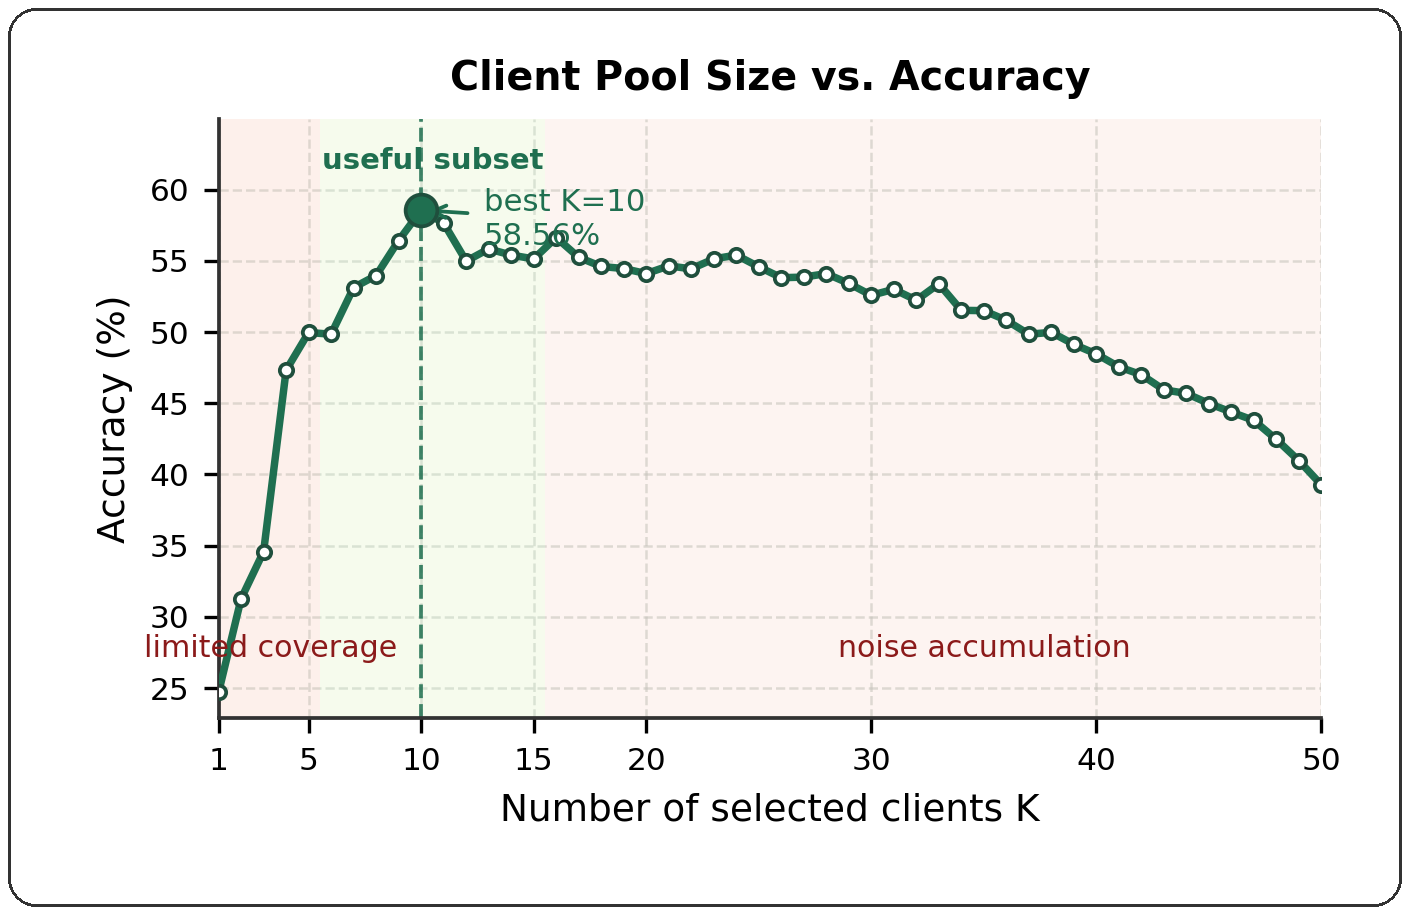
\includegraphics[width=\linewidth]{figure/scale_exp/top50-intro.png}
    \caption{\small Final test accuracy with different numbers of admitted clients under noisy and Non-IID settings. 
The result illustrates a non-monotonic trend: too few clients provide insufficient coverage, whereas too many clients introduce accumulated noise. 
A balanced subset yields the best accuracy.}
    \label{fig:top50-intro}
\end{figure}

\begin{figure*}[t]
\centering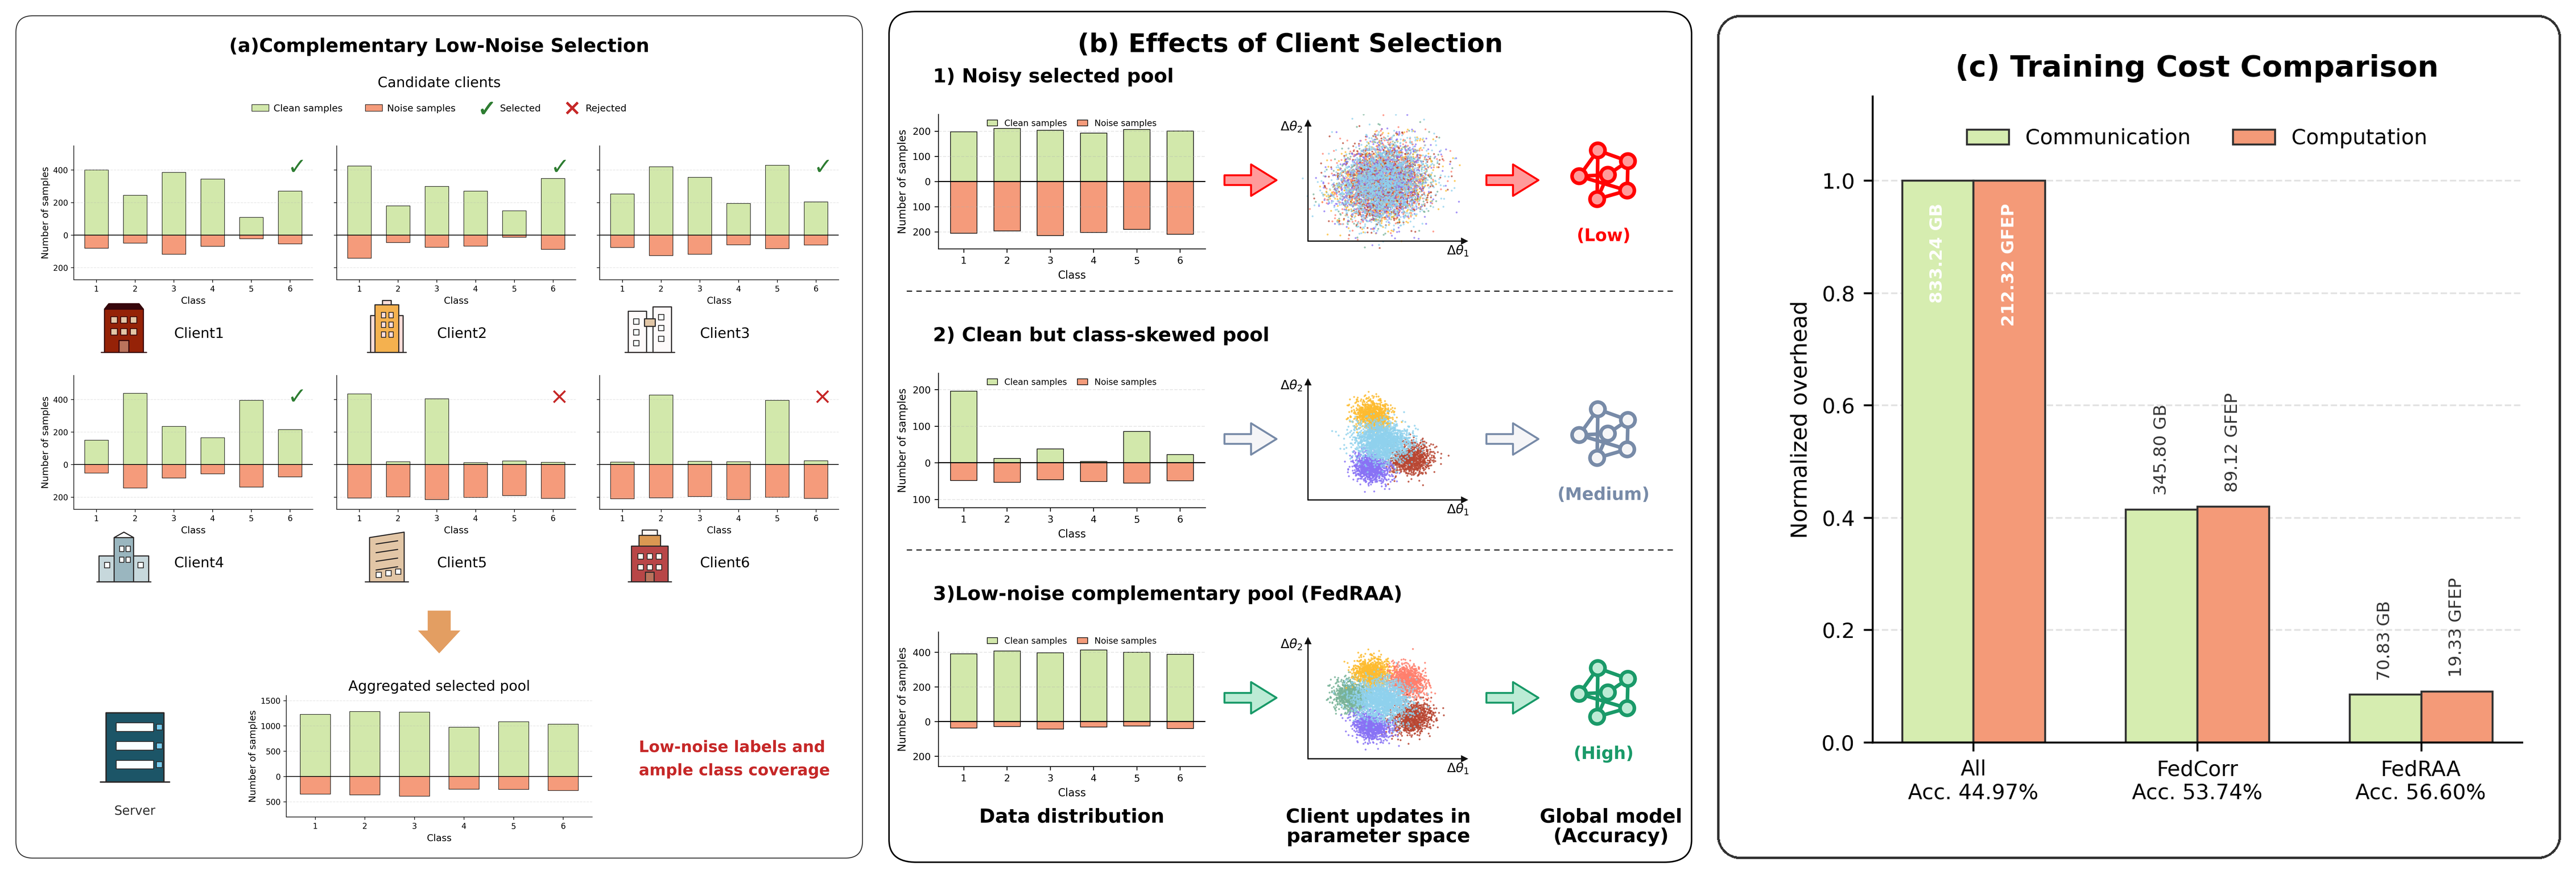
\includegraphics[width=\linewidth]{figure/display.png}
\caption{
Motivation and effect of FedRAA under heterogeneous noisy-label federated learning.
(a) Individual clients may be class-skewed and contain different amounts of label noise, while FedRAA selects a low-noise complementary subset whose aggregated distribution better covers all classes.
(b) Different selection outcomes lead to different update quality and final performance: noisy pools produce corrupted updates, clean but skewed pools induce biased representations, and the proposed low-noise complementary selection yields more robust global updates.
(c) Compared with representative baselines, FedRAA achieves higher accuracy while substantially reducing communication and computation overhead.
}\label{fig:display}\end{figure*}
Federated learning (FL) is often deployed in settings where the server faces a pool of candidate clients rather than a set of uniformly trustworthy participants~\cite{mcmahan2017communication,kairouz2021advances}. 
This is especially common in cross-institutional medical and real-world collaborative learning, where hospitals or sites differ in acquisition protocols, annotation quality, patient populations, and class distributions~\cite{rieke2020future,rehman2023federated,sandhu2023medical}. 
Because raw data remain local, the server cannot directly inspect or clean each client's dataset before training.
The practical question is therefore not only how to train a robust global model, but also \emph{which clients should be admitted into training in the first place}.

This question becomes difficult when label noise and Non-IID heterogeneity are coupled across clients.
A client with many samples may still be harmful if its labels are unreliable, while a clean client may be insufficient if it covers only a narrow part of the target distribution.
Thus, admitting more clients does not necessarily provide better training data.
Fig.~\ref{fig:top50-intro} illustrates this effect: final accuracy first improves as more clients are admitted, but then drops when additional clients introduce accumulated noise.
The best participant pool is neither the smallest nor the largest one, but a subset that is simultaneously reliable and representative.

Most existing robust FL methods act after clients have already entered the training process.
Round-level client selection schedules participants during training~\cite{cho2022power,oort,tang2022fedcor}; noisy-label FL methods correct or suppress corrupted supervision during local optimization~\cite{xu2022fedcorr,hao2025fedcs,sivasubramanian2024gcfl}; and robust aggregation filters abnormal updates on the server side~\cite{li2024feddiv,ACFL}.
These approaches are useful, but they inherit a post-admission limitation: persistently noisy or target-mismatched clients may repeatedly consume communication and computation resources before their influence is corrected.
When unreliable clients are caused by stable local data characteristics, repeatedly repairing their updates can be less efficient than preventing them from entering the training pool.

We therefore study \emph{pre-training client admission} for robust federated learning.
As shown in Fig.~\ref{fig:display}, the goal is to construct a ``golden client subset'' before federated communication begins.
This subset should exclude clients that are likely to inject noisy updates, while retaining enough distributional coverage to avoid a clean but biased training pool.
The central challenge is that this decision must be made under the privacy constraints of FL: the server cannot directly access, inspect, or relabel clients' raw samples to determine whether their data are useful.
Thus, unlike ordinary data selection, client admission must infer both data reliability and distributional contribution from privacy-compatible proxy signals.

To address this challenge, we propose \textbf{FedRAA}, a reliability- and representativeness-aware admission framework for FL under coupled label noise and Non-IID heterogeneity.
FedRAA first decides the participant pool using only proxy-based evidence, and standard federated training is then performed within this pool.
Specifically, FedRAA estimates client reliability using predictive entropy on a server-held proxy dataset, where higher uncertainty indicates higher label-noise risk~\cite{natarajan2013learning,tsouvalas2022labeling}.
It then measures subset-level representativeness by the KL divergence between the selected-client distribution and the proxy distribution~\cite{ben2010theory,hsu2019measuring,zhu2021survey,zhang2023dpp}.
Starting from a unified target-risk bound, we show that these two quantities correspond to the two key risks of an admitted subset: label-noise contamination and target-distribution mismatch.
By combining the two signals with a greedy admission strategy, FedRAA selects a low-noise and complementary client subset before federated optimization.

Our main contributions are summarized as follows:
\begin{itemize}
    \item We study robust federated learning from a pre-training client admission perspective under coupled label noise and Non-IID heterogeneity, and formulate the problem as golden client subset construction.

    \item We provide a unified target-risk upper bound that reveals two key subset-dependent factors, namely label-noise risk and distribution mismatch, thereby theoretically motivating reliable and representative client admission.

    \item We propose \textbf{FedRAA}, which combines proxy-set predictive entropy and KL-based distribution matching to select reliable and complementary clients before federated training. 
    Extensive experiments validate the theoretical motivation and show that FedRAA provides competitive robust accuracy with lower cost at matched target utility.
\end{itemize}

\section{Related Work}

\paragraph{Robust federated learning under unreliable clients.}
Federated learning is vulnerable to unreliable client updates caused by noisy labels, heterogeneous data distributions, or abnormal local training behavior.
Existing robust FL methods usually mitigate such risks after clients have already participated in training.
Noisy-label FL methods perform label correction, sample reweighting, small-loss selection, or local data refinement to reduce the influence of corrupted supervision~\cite{natarajan2013learning,tsouvalas2022labeling,xu2022fedcorr,liang2023fednoisy,hao2025fedcs,sivasubramanian2024gcfl}.
Robust aggregation and Byzantine-resilient defenses instead suppress abnormal updates at the server side~\cite{pillutla2022robust,yin2018byzantine,cao2021fltrust}.
These methods improve robustness during optimization, but they generally assume that potentially unreliable clients have already entered the training process.
When client unreliability is persistent, such as client-level label noise or target-mismatched data, repeatedly correcting or filtering their updates can still consume substantial communication and computation resources.
FedRAA addresses this issue from a different stage: it aims to reduce the risk of the participant pool before federated optimization begins.

\paragraph{Client selection and client admission.}
Client selection has been widely studied to improve the efficiency and convergence of FL.
Representative methods select clients according to estimated utility, loss, gradient correlation, diversity, or cluster-level informativeness~\cite{lai2021oort,cho2022power,tang2022fedcor,zhang2023dpp,ACFL}.
Most of these methods are designed for round-wise scheduling, where the server repeatedly chooses a subset of clients for the current communication round.
This setting differs from pre-training admission.
Round-wise scheduling asks which clients are useful at a particular optimization step, whereas admission asks whether a candidate client should be included in the training pool at all.
This distinction is important under coupled label noise and Non-IID heterogeneity: high loss, large gradients, or distributional diversity may indicate either useful hard examples or harmful corrupted supervision.
FedRAA therefore formulates client selection as a one-shot admission problem and evaluates clients according to their reliability and their contribution to the selected subset's distributional coverage.

\paragraph{Proxy-based reliability and representativeness.}
Because FL prevents the server from directly inspecting clients' raw data, pre-training admission must rely on privacy-compatible proxy signals.
Predictive uncertainty and entropy have been widely used as indicators of model confidence and can reflect the effect of corrupted supervision~\cite{natarajan2013learning,tsouvalas2022labeling}.
Meanwhile, distribution mismatch is a key factor in generalization under domain shift and Non-IID learning~\cite{ben2010theory,hsu2019measuring,zhu2021survey}.
These two lines of work motivate the two criteria used in FedRAA.
Specifically, FedRAA uses predictive entropy on a server-held proxy set to estimate client-level reliability, and KL-based proxy distribution matching to measure subset-level representativeness.
Different from methods that optimize either robustness or diversity alone, FedRAA combines both signals under a unified target-risk view, thereby selecting a low-noise and distributionally complementary client subset before training.


\section{Theoretical Analysis}
\label{sec:theoretical_analysis}

We study \emph{one-shot client admission} before federated optimization starts.
Rather than deciding whom to sample at every communication round, we first construct a participant pool from $N$ candidate clients and then run standard federated training within this pool.
The goal is to retain clients that are both \emph{reliable}, in the sense of having low predictive unreliability or low risk of corrupted supervision, and \emph{representative}, in the sense of being aligned with the target distribution seen by the server at test time.

\subsection{Problem Setup}
\label{subsec:problem_setup}

Let $P_T$ denote the target test distribution.
For any hypothesis $h\in\mathcal H$, its target risk is
\begin{equation}
\label{eq:target_risk_def}
\epsilon_T(h)
=
\mathbb E_{(x,y)\sim P_T}
\left[
\ell(h(x),y)
\right].
\end{equation}
% \begin{assumption}[Full participation after admission]
% Given a candidate client pool $\mathcal{C}$, an admitted subset 
% $\mathcal{S}\subseteq\mathcal{C}$ is determined before federated training starts. 
% During training, all clients in $\mathcal{S}$ participate in every communication round, and no round-wise client sampling or scheduling is performed.
% \end{assumption}
\begin{assumption}[Existence of risk-prone clients]
\label{assump:risk_prone_clients}
The candidate client pool $\mathcal{C}$ contains a non-empty subset of risk-prone clients 
$\mathcal{C}_{\mathrm{risk}}\subset \mathcal{C}$. 
Clients in $\mathcal{C}_{\mathrm{risk}}$ have persistent risks, such as severe label noise or distributional bias, which can repeatedly affect global aggregation once they are admitted to training.
\end{assumption}

\begin{definition}[Block-constrained sample subset in FL]
\label{def:block_constrained_subset}
Consider a federated system with $N$ candidate clients.
The global training set is partitioned into client blocks,
$D=\bigsqcup_{i=1}^{N}D_i$, where $D_i$ is the local dataset of client $i$.
From our perspective, the server cannot freely select arbitrary samples from $D$; instead, the feasible training subsets are restricted to unions of client blocks:
\[
D_S=\bigsqcup_{i\in S}D_i,
\qquad
\emptyset\neq S\subseteq  \mathcal{C}.
\]
Let $h_S$ denote the global model trained using the data blocks indexed by $S$.
The block-constrained optimal subset is
\begin{equation}
\label{eq:block_constrained_optimum}
S^\star
\in
\arg\min_{\emptyset\neq S\subseteq \mathcal{C}}
\epsilon_T(h_S).
\end{equation}
Here, $S^\star$ denotes the block-constrained optimal admitted subset. 
Ideally, the candidate pool can be decomposed into the admitted golden client subset and the risk-prone clients, i.e.,
\[
\mathcal{C}=S^\star\cup\mathcal{C}_{\mathrm{risk}}.
\]
Our goal is to approximate the block-constrained optimum in Eq.~\eqref{eq:block_constrained_optimum} through a computable pre-training admission rule.
\end{definition}

\subsection{A Unified Risk View of Client Admission}
\label{subsec:risk_view}

We provide a risk-based justification for pre-training client admission.
In our formulation, each client is treated as an indivisible data block; therefore, changing the admitted set $S$ changes the training distribution induced by the selected local datasets.
Under noisy and heterogeneous settings, this induced distribution may suffer from label corruption and target-distribution mismatch.
We show that both factors enter an upper bound on the target risk, thereby motivating reliability- and representativeness-aware client admission.

\begin{assumption}[Bounded loss]
\label{assump:bounded_loss}
The loss function is bounded:
\begin{equation}
0\le \ell(h(x),y)\le 1,
\qquad
\forall h\in\mathcal{H},\ (x,y)\in\mathcal{X}\times\mathcal{Y}.
\end{equation}
\end{assumption}

\begin{assumption}[Label-shift-dominated heterogeneity]
\label{assump:label_shift}
For every clean client distribution $\mu_i$ and the target distribution $P_T$, the class-conditional distribution is shared:
\begin{equation}
\mu_i(x,y)=p(x\mid y)q_i(y),
\qquad
P_T(x,y)=p(x\mid y)q_T(y),
\end{equation}
where $q_i\in\Delta^{K-1}$ is the clean label prior of client $i$, and $q_T\in\Delta^{K-1}$ is the target label prior.
\end{assumption}

Assumption~\ref{assump:label_shift} focuses on label-prior heterogeneity, where clients differ mainly in class proportions rather than in class-conditional feature distributions.
Thus, the theoretical bound characterizes a label-shift-dominated case of Non-IID FL.
More general forms of heterogeneity, such as feature shift or domain shift, are evaluated empirically but are not fully covered by this simplified analysis.

For a selected subset $S$, define its clean mixture label prior as
\begin{equation}
\bar q_S
=
\sum_{i\in S}w_i(S)q_i,
\qquad
w_i(S)=\frac{n_i}{\sum_{j\in S}n_j}.
\end{equation}
Under Assumption~\ref{assump:label_shift}, the clean selected-client mixture can be written as
\begin{equation}
P_S^c(x,y)=p(x\mid y)\bar q_S(y).
\end{equation}

\begin{assumption}[Label-only noise]
\label{assump:label_only_noise}
For any selected subset $S$, the clean selected-client mixture $P_S^c(X,Y)$ and the noisy selected-client mixture $P_S^n(X,\widetilde Y)$ share the same input marginal:
\begin{equation}
P_S^c(X)=P_S^n(X).
\end{equation}
That is, label noise only corrupts the clean label $Y$ into the observed label $\widetilde Y$.
\end{assumption}

Define the posterior label-noise discrepancy as
\begin{equation}
\label{eq:posterior_noise_discrepancy}
\xi_{\mathrm{noise}}(S)
=
\mathbb{E}_{x\sim P_S^X}
\left[
\sum_{c=1}^{K}
\left|
P_S^c(Y=c\mid x)
-
P_S^n(\widetilde Y=c\mid x)
\right|
\right].
\end{equation}

\begin{lemma}[Posterior-noise decomposition]
\label{lem:noise_bridge}
Under Assumptions~\ref{assump:bounded_loss} and~\ref{assump:label_only_noise}, 
for any $h\in\mathcal H$ and any selected subset $S$, let
$\epsilon_S^c(h)$ and $\epsilon_S^n(h)$ denote the clean and noisy risks on $S$, respectively. Then,
\begin{equation}
\label{eq:clean_noisy_bridge}
\left|
\epsilon_S^c(h)-\epsilon_S^n(h)
\right|
\le
\xi_{\mathrm{noise}}(S).
\end{equation}
Consequently,
\begin{equation}
\epsilon_S^c(h)
\le
\epsilon_S^n(h)
+
\xi_{\mathrm{noise}}(S).
\end{equation}
\end{lemma}

This lemma should be interpreted as a risk decomposition showing how label corruption enters the target-risk bound.
It does not claim that the posterior discrepancy in Eq.~\eqref{eq:posterior_noise_discrepancy} is directly observable by the server.

\begin{lemma}[Clean target-transfer under label shift]
\label{lem:label_shift_transfer}
Under Assumptions~\ref{assump:bounded_loss} and~\ref{assump:label_shift}, for any $h\in\mathcal{H}$ and any selected subset $S$,
\begin{equation}
\label{eq:clean_transfer}
\epsilon_T(h)
\le
\epsilon_S^c(h)
+
\frac{1}{2}\|\bar q_S-q_T\|_1.
\end{equation}
\end{lemma}



\begin{theorem}[Unified admission risk bound]
\label{thm:main_bound}
Combining Lemma~\ref{lem:label_shift_transfer} with Lemma~\ref{lem:noise_bridge}, we obtain that, for any selected subset $S$ and any $h\in\mathcal{H}$,
\begin{equation}
\label{eq:main_bound}
\epsilon_T(h)
\le
\epsilon_S^n(h)
+
\xi_{\mathrm{noise}}(S)
+
\frac{1}{2}\|\bar q_S-q_T\|_1.
\end{equation}
\end{theorem}

Theorem~\ref{thm:main_bound} shows that the target risk is controlled by two subset-dependent quantities: the noise-contamination term $\xi_{\mathrm{noise}}(S)$ and the distribution-mismatch term $\|\bar q_S-q_T\|_1$.
Thus, client admission is not merely a heuristic pre-processing step; changing $S$ directly changes the upper bound on the target risk.

\subsection{From Population Bound to Proxy Admission Surrogates}
\label{subsec:proxy_theory}

The bound in Theorem~\ref{thm:main_bound} contains population quantities that are not directly observable before training.
In particular, $\xi_{\mathrm{noise}}(S)$ depends on the discrepancy between clean and noisy label posteriors, while $\bar q_S$ and $q_T$ are clean population label priors.
Therefore, FedRAA cannot directly optimize the population bound.
Instead, we introduce observable proxy statistics and explicitly account for their approximation residuals.
This section should be interpreted as a conditional bridge from the population-level bound to the proxy objective used by the algorithm.

\begin{figure}
    \centering
    
\includegraphics[width=\linewidth]{figure/熵值曲线/3合1.png}
    \caption{Predictive entropy provides an effective signal for characterizing client-side noise conditions. We report the entropy--noise rate curves on CIFAR-10, CIFAR-100, and TinyImageNet, together with the corresponding normalized mutual information. The results demonstrate that predictive entropy can reliably reflect the variation of noise rates across clients, supporting its use as a lightweight criterion for noisy-client identification.}
    \label{fig:entropy}
\end{figure}

First, we choose predictive entropy as our noise proxy objective. As shown in Figure~\ref{fig:entropy}, predictive entropy is correlated with the client-side noise rate. Clients with higher label noise generally produce more uncertain predictions on the proxy set, leading to larger entropy values. Based on this empirical evidence, we adopt predictive entropy as a lightweight proxy for quantifying client reliability during training.

Let $\widetilde H_i\in[0,1]$ be the normalized predictive entropy of client $i$ on the proxy set, and define the entropy-based set-level proxy
\begin{equation}
\label{eq:entropy_proxy_set}
\widehat{\xi}_{H}(S)
=
\sum_{i\in S}
\omega_i(S)\widetilde H_i,
\qquad
\omega_i(S)=\frac{n_i}{\sum_{j\in S}n_j}.
\end{equation}
Let $z_S$ be the proxy-predicted class mixture of the selected client set, and let $p_{\mathrm{proxy}}$ denote the empirical label distribution of the server proxy set.
For numerical stability, define the smoothed mixture
\begin{equation}
\label{eq:smoothed_proxy_mixture}
z_S^\epsilon
=
\frac{z_S+\epsilon \mathbf 1}{1+K\epsilon}.
\end{equation}

Rather than assuming that these proxies are exact, we define the following residual terms:
\begin{align}
\label{eq:entropy_residual}
r_H(S;c_H)
&=
\left[
\xi_{\mathrm{noise}}(S)
-
c_H\widehat{\xi}_{H}(S)
\right]_+,\\
\label{eq:coverage_residual}
r_Z(S)
&=
\frac12\|\bar q_S-z_S\|_1,\\
\label{eq:target_proxy_residual}
r_T
&=
\frac12\|p_{\mathrm{proxy}}-q_T\|_1,\\
\label{eq:smoothing_residual}
r_\epsilon(S)
&=
\frac12\|z_S-z_S^\epsilon\|_1,
\end{align}
where $[a]_+=\max\{a,0\}$ and $c_H>0$ is a scaling constant.
Here, $r_H$ measures the gap between the population noise-contamination term and the entropy-based proxy, $r_Z$ measures the mismatch between the proxy-predicted mixture and the clean selected-client prior, $r_T$ measures the mismatch between the proxy label distribution and the target prior, and $r_\epsilon$ accounts for smoothing.

\begin{theorem}[Residualized proxy admission bound]
\label{thm:residualized_proxy_bound}
Under Assumptions~\ref{assump:bounded_loss}--\ref{assump:label_only_noise}, for any selected subset $S$, any $h\in\mathcal H$, and any $c_H>0$,
\begin{equation}
\label{eq:residualized_proxy_bound}
\epsilon_T(h)
\le
\epsilon_S^n(h)
+
c_H\widehat{\xi}_{H}(S)
+
\sqrt{
\frac12
\mathrm{KL}
\left(
p_{\mathrm{proxy}}\|z_S^\epsilon
\right)
}
+
R_{\mathrm{proxy}}(S;c_H),
\end{equation}
where
\begin{equation}
\label{eq:proxy_residual_total}
R_{\mathrm{proxy}}(S;c_H)
=
r_H(S;c_H)
+
r_Z(S)
+
r_T
+
r_\epsilon(S).
\end{equation}
\end{theorem}

Theorem~\ref{thm:residualized_proxy_bound} does not assume that predictive entropy or proxy-predicted signatures are universally accurate.
Instead, it separates the observable part of the bound from the residual terms that quantify proxy mismatch.
Thus, FedRAA optimizes the observable surrogate, while $R_{\mathrm{proxy}}(S;c_H)$ captures the remaining gap between proxy statistics and population quantities.

\begin{corollary}[Proxy-consistency admission surrogate]
\label{cor:proxy_consistency_surrogate}
Suppose that the proxy residual is uniformly bounded over the candidate subsets under consideration, i.e.,
$R_{\mathrm{proxy}}(S;c_H)\le \delta_{\mathrm{proxy}}$.
Then, for any $\lambda_s>0$,
\begin{equation}
\label{eq:proxy_consistency_bound}
\epsilon_T(h)
\le
\epsilon_S^n(h)
+
c_H\widehat{\xi}_{H}(S)
+
\lambda_s
\mathrm{KL}
\left(
p_{\mathrm{proxy}}\|z_S^\epsilon
\right)
+
\delta_{\mathrm{proxy}}
+
\frac{1}{8\lambda_s}.
\end{equation}
\end{corollary}

Corollary~\ref{cor:proxy_consistency_surrogate} motivates the computable subset-level admission surrogate
\begin{equation}
\label{eq:proxy_surrogate_objective}
\widehat{\mathcal B}(S)
=
\lambda_m\widehat{\xi}_{H}(S)
+
\lambda_s
\mathrm{KL}
\left(
p_{\mathrm{proxy}}\|z_S^\epsilon
\right),
\end{equation}
where $\lambda_m$ absorbs the unknown scaling constant $c_H$.
This surrogate is the observable part of the residualized proxy bound.
The residual terms are not directly optimized by FedRAA; they characterize the approximation gap introduced by using proxy statistics.
Accordingly, the theory should be interpreted as a conditional justification: when the proxy residuals are small, minimizing the entropy--KL surrogate controls the target-risk bound. Additional discussion is provided in Appendix~\ref{app:entropy_residual}--\ref{app:smoothing_residual}.

\section{Method}
\label{sec:method}

The theoretical analysis motivates an additive proxy objective consisting of an entropy-based predictive unreliability term and a proxy distribution-mismatch term.
FedRAA implements this objective in four layers.
First, we instantiate the theory-derived proxy objective using normalized predictive entropy and proxy-KL matching.
Second, we convert the additive objective into a local candidate-wise score for greedy admission.
Third, we optionally apply noise-adaptive exponents as a practical calibration mechanism.
Finally, we use a variable-size prefix rule to determine how many clients to admit.
Only the first two layers are directly tied to the proxy objective; the adaptive exponent and prefix-threshold mechanisms are practical choices for robustness under heterogeneous noise.

\subsection{Reliability Surrogate via Fixed-Scale Predictive Entropy}
\label{subsec:reliability_surrogate}

Before admission, each candidate client starts from the current global model and performs a short local adaptation, producing a client model $f_i$.
This adaptation is performed once before federated training, using a small fixed local budget $E_{\mathrm{adm}}$, and all candidate clients follow the same protocol.
It introduces a one-time pre-screening cost, but avoids repeatedly auditing unreliable clients during later communication rounds.

Let $p_i(c\mid x)$ denote the predictive probability of client model $f_i$ on proxy input $x\in\mathcal D_{\mathrm{proxy}}$.
We define the average predictive entropy of client $i$ as
\begin{equation}
\label{eq:entropy_main}
H_i
=
-\frac{1}{|\mathcal D_{\mathrm{proxy}}|}
\sum_{x\in\mathcal D_{\mathrm{proxy}}}
\sum_{c=1}^{K}
p_i(c\mid x)\log p_i(c\mid x).
\end{equation}
For a $K$-class categorical distribution, the maximum entropy is $\log K$, achieved by the uniform distribution.
We therefore normalize $H_i$ as $\widetilde H_i=H_i/\log K$, so that $\widetilde H_i\in[0,1]$ in theory.
A value close to $1$ indicates near-uniform predictive uncertainty on the proxy set, which we use as an observable proxy for predictive unreliability.
In implementation, $\widetilde H_i$ is clipped to $[0,1]$ only for numerical stability.

The fixed-scale reliability score is
\begin{equation}
\label{eq:quality_score}
C_m(i)
=
\max\{1-\widetilde H_i,\epsilon\},
\end{equation}
where $\epsilon>0$ prevents zero reliability and keeps the negative-log cost finite.
At the set level, this score corresponds to the entropy-based proxy term $\widehat{\xi}_{H}(S)=\sum_{i\in S}\omega_i(S)\widetilde H_i$, where $\omega_i(S)=n_i/\sum_{j\in S}n_j$.
Thus, selecting clients with larger $C_m(i)$ discourages the admitted set from accumulating high estimated predictive unreliability.

\subsection{Representativeness Surrogate via Proxy-Predicted Class Signatures}
\label{subsec:representativeness_surrogate}

Let $p_{\mathrm{proxy}}\in\Delta^{K-1}$ be the empirical label distribution of $\mathcal D_{\mathrm{proxy}}$.
For each client $i$, we construct a proxy-predicted class signature from hard predictions:
\begin{equation}
\label{eq:predictive_signature_main}
r_i(c)
=
\sum_{x\in\mathcal D_{\mathrm{proxy}}}
\mathbf{1}
\left[
\arg\max_{c'}p_i(c'\mid x)=c
\right],
\qquad c=1,\dots,K.
\end{equation}
Let $\hat r_i=r_i/(\sum_{c=1}^{K}r_i(c)+\epsilon)$ denote the normalized signature.
For a selected subset $S$, we define the proxy-predicted mixture as
\begin{equation}
\label{eq:subset_signature_main}
z_S
=
\sum_{i\in S}
\omega_i(S)\hat r_i
\in\Delta^{K-1},
\qquad
\omega_i(S)=\frac{n_i}{\sum_{j\in S}n_j}.
\end{equation}
This weighted form mirrors the clean mixture prior $\bar q_S=\sum_{i\in S}w_i(S)q_i$ in the theoretical analysis, while replacing the unobservable clean prior $q_i$ with the observable proxy-predicted signature $\hat r_i$.
Operationally, $z_S$ is better interpreted as the target-facing predictive coverage of the admitted client pool, rather than an exact estimate of the clients' true clean label priors.

For numerical stability, we apply $\epsilon$-smoothing before computing KL divergence:
\[
z_S^\epsilon=\frac{z_S+\epsilon\mathbf 1}{1+K\epsilon}.
\]
For a candidate client $k\notin S$, we measure the distribution mismatch after admitting $k$ by $d(k\mid S)=\mathrm{KL}(p_{\mathrm{proxy}}\|z_{S\cup\{k\}}^\epsilon)$ and convert it into the distribution score
\begin{equation}
\label{eq:distribution_score}
C_s(k\mid S)
=
\exp\!\left(-\tau d(k\mid S)\right).
\end{equation}
We use the forward direction $\mathrm{KL}(p_{\mathrm{proxy}}\|z_{S\cup\{k\}}^\epsilon)$ because missing proxy target classes in the admitted pool should be penalized strongly.
When $\tau$ is not fixed, we calibrate it from the valid candidate pool $\mathcal V$ by setting $\tau=(Q_{q_\tau}(\{d(i\mid\emptyset):i\in\mathcal V\})+\epsilon)^{-1}$.
This calibration makes the score less sensitive to the absolute KL scale of a particular dataset or candidate pool.

\subsection{From Additive Surrogate to Local Admission Score}
\label{subsec:local_admission_score}

The additive proxy objective in Eq.~\eqref{eq:proxy_surrogate_objective} is a set-level objective.
FedRAA does not solve this combinatorial problem exactly.
Instead, it greedily minimizes a local candidate-wise approximation.
For a candidate client $k\notin S$, the post-admission KL term $\mathrm{KL}(p_{\mathrm{proxy}}\|z_{S\cup\{k\}}^\epsilon)$ measures the distribution mismatch after admitting $k$, while the entropy term $\widetilde H_k$ serves as a local approximation to the marginal increase of the set-level unreliability term.

A direct fixed-score implementation of the additive surrogate is
\begin{equation}
\label{eq:fixed_admission_score}
A_0(k\mid S)
=
\exp
\left(
-\lambda_s
\mathrm{KL}
\left(
p_{\mathrm{proxy}}\|z_{S\cup\{k\}}^\epsilon
\right)
-
\lambda_m\widetilde H_k
\right).
\end{equation}
This score directly exponentiates the additive surrogate. Since the exponential
of a weighted sum factorizes into a product, Eq.~\eqref{eq:fixed_admission_score}
naturally motivates a multiplicative score over the two components. Using the
bounded monotone scores defined above, namely $C_s(k\mid S)$ in
Eq.~\eqref{eq:distribution_score} and $C_m(k)$ in Eq.~\eqref{eq:quality_score},
we obtain the practical admission utility
\begin{equation}
\label{eq:adaptive_utility}
A(k\mid S)
=
C_s(k\mid S)^{a_{\mathrm{eff}}}
C_m(k)^{b_{\mathrm{eff}}}.
\end{equation}
This form preserves the preference direction of the additive surrogate while
keeping both factors bounded and numerically stable. Fixed exponents give the
non-adaptive version, whereas adaptive exponents reweight the two components
during admission.


The multiplicative form is conservative: a client must be both distributionally useful and sufficiently reliable to obtain a high score.
Equivalently, maximizing $A(k\mid S)$ is minimizing the negative-log admission cost
\begin{align}
\label{eq:admission_cost}
R(k\mid S)
&=
-\log A(k\mid S)\\
&=
a_{\mathrm{eff}}\tau
\mathrm{KL}\!\left(p_{\mathrm{proxy}}\|z_{S\cup\{k\}}^\epsilon\right)
+
b_{\mathrm{eff}}\big[-\log C_m(k)\big].
\end{align}
Eq.~\eqref{eq:admission_cost} can be viewed as a local candidate-wise negative-log approximation to Eq.~\eqref{eq:proxy_surrogate_objective}, with $-\log C_m(k)$ replacing the marginal entropy cost and the forward KL measuring the post-admission distribution mismatch.
For small to moderate entropy values, $-\log(1-\widetilde H_k)\approx \widetilde H_k$, while highly uncertain clients receive a stronger penalty.

\subsection{Optional Noise-Adaptive Calibration}
\label{subsec:adaptive_calibration}

The adaptive exponents are practical calibration terms, not a direct consequence of the risk bound.
The core theory-aligned version uses fixed weights in Eq.~\eqref{eq:fixed_admission_score}.
However, a fixed reliability--representativeness trade-off can be suboptimal under heterogeneous noise.
When the candidate pool is severely noisy, admission should emphasize reliability; when the pool is moderately noisy, representativeness becomes more important for target-distribution coverage.

We estimate the global predictive unreliability level from normalized entropy scores:
\begin{equation}
\label{eq:global_noise_score}
s
=
\rho\,\mathrm{Mean}(\{\widetilde H_i\}_{i\in\mathcal V})
+
(1-\rho)\,Q_q(\{\widetilde H_i\}_{i\in\mathcal V}),
\qquad
\rho\in[0,1].
\end{equation}
Given $s$, define $g=\mathrm{clip}(2(0.5-s),-1,1)$.
Let $a$ and $b$ be base exponents.
We use $a_{\mathrm{eff}}=\mathrm{clip}(a(1+\lambda g),a_{\min},a_{\max})$ and $\bar b_{\mathrm{eff}}=\mathrm{clip}(b(1-\lambda g),b_{\min},b_{\max})$.
For datasets with many classes, entropy is harder to calibrate; hence we use the class-scaled exponent $b_{\mathrm{eff}}=\bar b_{\mathrm{eff}}(\max\{K/K_b,1\})^{-\nu_b}$, where $K_b$ is a reference class number and $\nu_b\ge0$ controls the scaling strength.
When $s>0.5$, $g<0$, so $a_{\mathrm{eff}}$ decreases and $b_{\mathrm{eff}}$ increases; the admission rule emphasizes reliability under severe uncertainty.
When $s<0.5$, the rule increases the distribution weight and encourages broader target-distribution coverage.
We evaluate the fixed-score variant and the adaptive variant separately in the ablation study.

\subsection{Variable-Size Greedy Participant Construction}
\label{subsec:variable_greedy}

\begin{algorithm}[t]
\caption{FedRAA: Fixed-Scale Noise-Adaptive Client Admission}
\label{alg:FedRAA}
\begin{algorithmic}[1]
\Require Candidate clients $[N]$, sample sizes $\{n_i\}_{i=1}^N$, proxy dataset $\mathcal D_{\mathrm{proxy}}$, admission adaptation budget $E_{\mathrm{adm}}$, greedy horizon $M$, minimum budget $K_{\min}$, parameters $\rho,q,a,b,\lambda,\tau,q_\tau,\eta_{\min},\eta_{\max},\tau_K$
\Ensure Selected participant pool $S^\star$
\State $\mathcal V\leftarrow[N]$, $S_0\leftarrow\emptyset$, $J(S_0)\leftarrow0$
\For{$i\in\mathcal V$}
    \State Obtain client model $f_i$ after short local adaptation with budget $E_{\mathrm{adm}}$
    \State Compute predictive entropy $H_i$ by Eq.~\eqref{eq:entropy_main}
    \State Normalize entropy as $\widetilde H_i\leftarrow H_i/\log K$
    \State Compute reliability score $C_m(i)$ by Eq.~\eqref{eq:quality_score}
    \State Compute proxy-predicted signature $r_i$ by Eq.~\eqref{eq:predictive_signature_main}
\EndFor
\State Compute proxy label distribution $p_{\mathrm{proxy}}$
\State Compute global unreliability score $s$ by Eq.~\eqref{eq:global_noise_score}
\State Compute $a_{\mathrm{eff}}$ and $b_{\mathrm{eff}}$ as described in Section~\ref{subsec:adaptive_calibration}
\State Calibrate $\tau$ if not fixed, and compute adaptive benchmark $\eta(s,K;\tau_K)$ by Eq.~\eqref{eq:eta_temp}
\For{$m=1,\dots,\min(M,|\mathcal V|)$}
    \For{each $k\in\mathcal V\setminus S_{m-1}$}
        \State Form smoothed mixture $z_{S_{m-1}\cup\{k\}}^\epsilon$
        \State Compute $C_s(k\mid S_{m-1})$ by Eq.~\eqref{eq:distribution_score}
        \State Compute $A(k\mid S_{m-1})$ by Eq.~\eqref{eq:adaptive_utility}
    \EndFor
    \State $k_m\leftarrow\arg\max_{k\in\mathcal V\setminus S_{m-1}}A(k\mid S_{m-1})$
    \State $S_m\leftarrow S_{m-1}\cup\{k_m\}$
    \State $J(S_m)\leftarrow J(S_{m-1})+\log\frac{A(k_m\mid S_{m-1})}{\eta(s,K;\tau_K)}$
\EndFor
\State $S^\star\leftarrow \arg\max_{S_m:\,m\ge K_{\min}}J(S_m)$
\State \Return $S^\star$
\end{algorithmic}
\end{algorithm}

Many existing client selection methods assume a predefined per-round
participation budget, such as a fixed fraction or a fixed number of clients
\cite{mcmahan2017communication, lai2021oort, cho2022power}.
However, a fixed budget can be undesirable under heterogeneous noise.
If the budget is too large, the server may be forced to admit unreliable clients; if it is too small, useful and target-complementary clients may be discarded.
We therefore allow the final participant pool size to be determined by the admission sequence, and introduce a temperature coefficient to explicitly control the retained cardinality.

We use the full candidate pool $\mathcal V=[N]$.
FedRAA then constructs a greedy sequence $S_1\subset S_2\subset\cdots\subset S_M$, where $M$ is the greedy horizon.
At step $m$, the selected client is
\begin{equation}
\label{eq:greedy_step}
k_m
=
\arg\max_{k\in\mathcal V\setminus S_{m-1}}
A(k\mid S_{m-1}),
\qquad
S_m=S_{m-1}\cup\{k_m\}.
\end{equation}

The KL-based objective is not generally submodular, so the greedy rule should be viewed as a practical approximation rather than an approximation-guaranteed optimizer.
Its role is to construct a high-scoring admission sequence, from which the final pool size is selected by a noise-adaptive prefix objective.

To decide how many clients to admit, we use a noise-adaptive benchmark with a cardinality temperature coefficient $\tau_K>0$.
Given the global unreliability score $s$, define
\[
\eta_0(s)=\mathrm{clip}(\eta_{\min}+(\eta_{\max}-\eta_{\min})s,\epsilon,1),
\]
and
\begin{equation}
\label{eq:eta_temp}
\eta(s,K;\tau_K)
=
\mathrm{clip}\!\left(
\left[
\eta_0(s)\bigl(\max\{K/K_\eta,1\}\bigr)^{-\nu_\eta}
\right]^{\tau_K},
\epsilon,1
\right).
\end{equation}
A larger $s$ yields a stricter baseline; $\tau_K$ controls the selection aggressiveness.
Because the inner benchmark lies in $(0,1]$, larger $\tau_K$ decreases the effective admission threshold and tends to retain more clients, while smaller $\tau_K$ yields a more conservative pool.

For each prefix $S_m$, we compute the cumulative threshold-normalized objective
\begin{equation}
\label{eq:prefix_objective}
J(S_m)
=
\sum_{t=1}^{m}
\log
\frac{
A(k_t\mid S_{t-1})
}{
\eta(s,K;\tau_K)
}.
\end{equation}
Equivalently,
\[
J(S_m)=\sum_{t=1}^{m}\log A(k_t\mid S_{t-1})-m\log\eta(s,K;\tau_K),
\]
which is an accumulated admission utility with a noise-adaptive cardinality penalty.
Under a minimum client constraint $K_{\min}$, the final participant pool is
\begin{equation}
\label{eq:variable_size_selection}
S^\star
=
\arg\max_{S_m:\,m\ge K_{\min}}
J(S_m).
\end{equation}
This mechanism adapts the selected client count to the observed quality and distributional complementarity of the candidate pool.
In high-uncertainty regimes, the selected set can shrink to avoid unreliable clients; when the candidate pool is mostly reliable and complementary, the method can retain more useful clients.

% \paragraph{Complexity.}
% FedRAA introduces a one-time pre-training screening cost.
% Scoring candidates requires $O(|\mathcal V|E_{\mathrm{adm}})$ local adaptation cost, where $E_{\mathrm{adm}}$ is the short admission adaptation budget.
% Proxy evaluation requires $O(|\mathcal V||\mathcal D_{\mathrm{proxy}}|)$ forward passes.
% After proxy signatures are computed, each greedy step evaluates at most $|\mathcal V|$ candidates with $K$-dimensional class mixtures, giving $O(M|\mathcal V|K)$ scoring cost for a greedy horizon $M$.
% These costs are incurred once before federated optimization, rather than at every communication round.


Algorithm~\ref{alg:FedRAA} summarizes the complete FedRAA procedure.



\section{Experiments}
\label{sec:experiment}

We evaluate FedRAA from four complementary perspectives. 
First, an oracle experiment checks whether the risk factors in Theorem~\ref{thm:main_bound} explain the quality of admitted client subsets. 
Second, we compare FedRAA with noisy-label FL methods and client selection baselines under coupled label noise and Non-IID heterogeneity. 
Third, we analyze the selected client subsets to verify whether the admitted clients are both reliable and representative. 
Finally, ablation studies isolate the effects of the reliability score, the distribution score, and the noise-adaptive calibration mechanism.

\subsection{Oracle Experiment}
\label{subsec:oracle_exp}

To provide a controlled validation of our theoretical analysis, we design a small-scale oracle experiment in which the clean label prior and the label-noise rate of each client are explicitly specified. 
This experiment is not intended to compare FedRAA with practical baselines. 
Instead, its goal is to verify whether the two subset-dependent factors identified in Theorem~\ref{thm:main_bound}, namely label-noise risk and distribution mismatch, can explain the quality of different admitted client subsets.

\paragraph{Experimental Setup.}
We consider a three-class classification problem with two-dimensional input features. 
Each class is generated from a Gaussian distribution with shared covariance but different class means. 
The target distribution is class-balanced, while the six candidate clients differ in both label-prior distribution and label-noise rate. 
For each client, labels are corrupted by symmetric noise: with probability $\rho$, the true label is uniformly flipped to one of the other $K-1$ classes. 
The detailed configuration is summarized in Table~\ref{tab:oracle_setup}.

We compare four representative admission strategies:
\begin{itemize}
    \item \textbf{All clients}: all candidate clients are admitted without screening.
    \item \textbf{Clean-only skewed}: only low-noise clients are admitted.
    \item \textbf{Balanced noisy}: all class-balanced client subset is admitted.
    \item \textbf{FedRAA ideal}: clients that are both low-noise and distributionally complementary are admitted.
\end{itemize}
The first strategy corresponds to naive full admission, while the next two strategies isolate the effects of distribution mismatch and label noise, respectively. 
The last strategy represents the oracle version of the reliability- and representativeness-aware admission principle advocated by FedRAA.

\paragraph{Results.}
We first compute the theoretical upper bound derived in Theorem~\ref{thm:main_bound} for different admitted subsets. 
As shown in Fig.~\ref{fig:oracle_summary}, the FedRAA ideal subset achieves the lowest theoretical risk bound, since it simultaneously reduces the label-noise term and the distribution-mismatch term.
In contrast, the balanced noisy strategy leads to the largest bound, indicating that distributional balance alone is insufficient when the admitted clients contain severe label noise.

We further compare the empirical target risk with the corresponding theoretical upper bound during training. 
As shown in Fig.~\ref{fig:oracle_summary}, the FedRAA ideal subset achieves both the lowest target risk and the smallest gap between the empirical risk and the theoretical bound.
This result supports the validity of our theoretical analysis: a subset with low label-noise risk and small distribution mismatch is more likely to yield better target performance. 
Moreover, by comparing the clean-only skewed strategy with the balanced noisy strategy in Fig.~\ref{fig:oracle_summary}, we observe that label noise can be more harmful than label-prior skewness in this controlled setting.
This observation further motivates the dynamic weighting mechanism in FedRAA, 
where the contributions of reliability and representativeness are adjusted adaptively 
based on the noise characteristics of the candidate client pool.

\begin{figure*}[t]
    \centering
    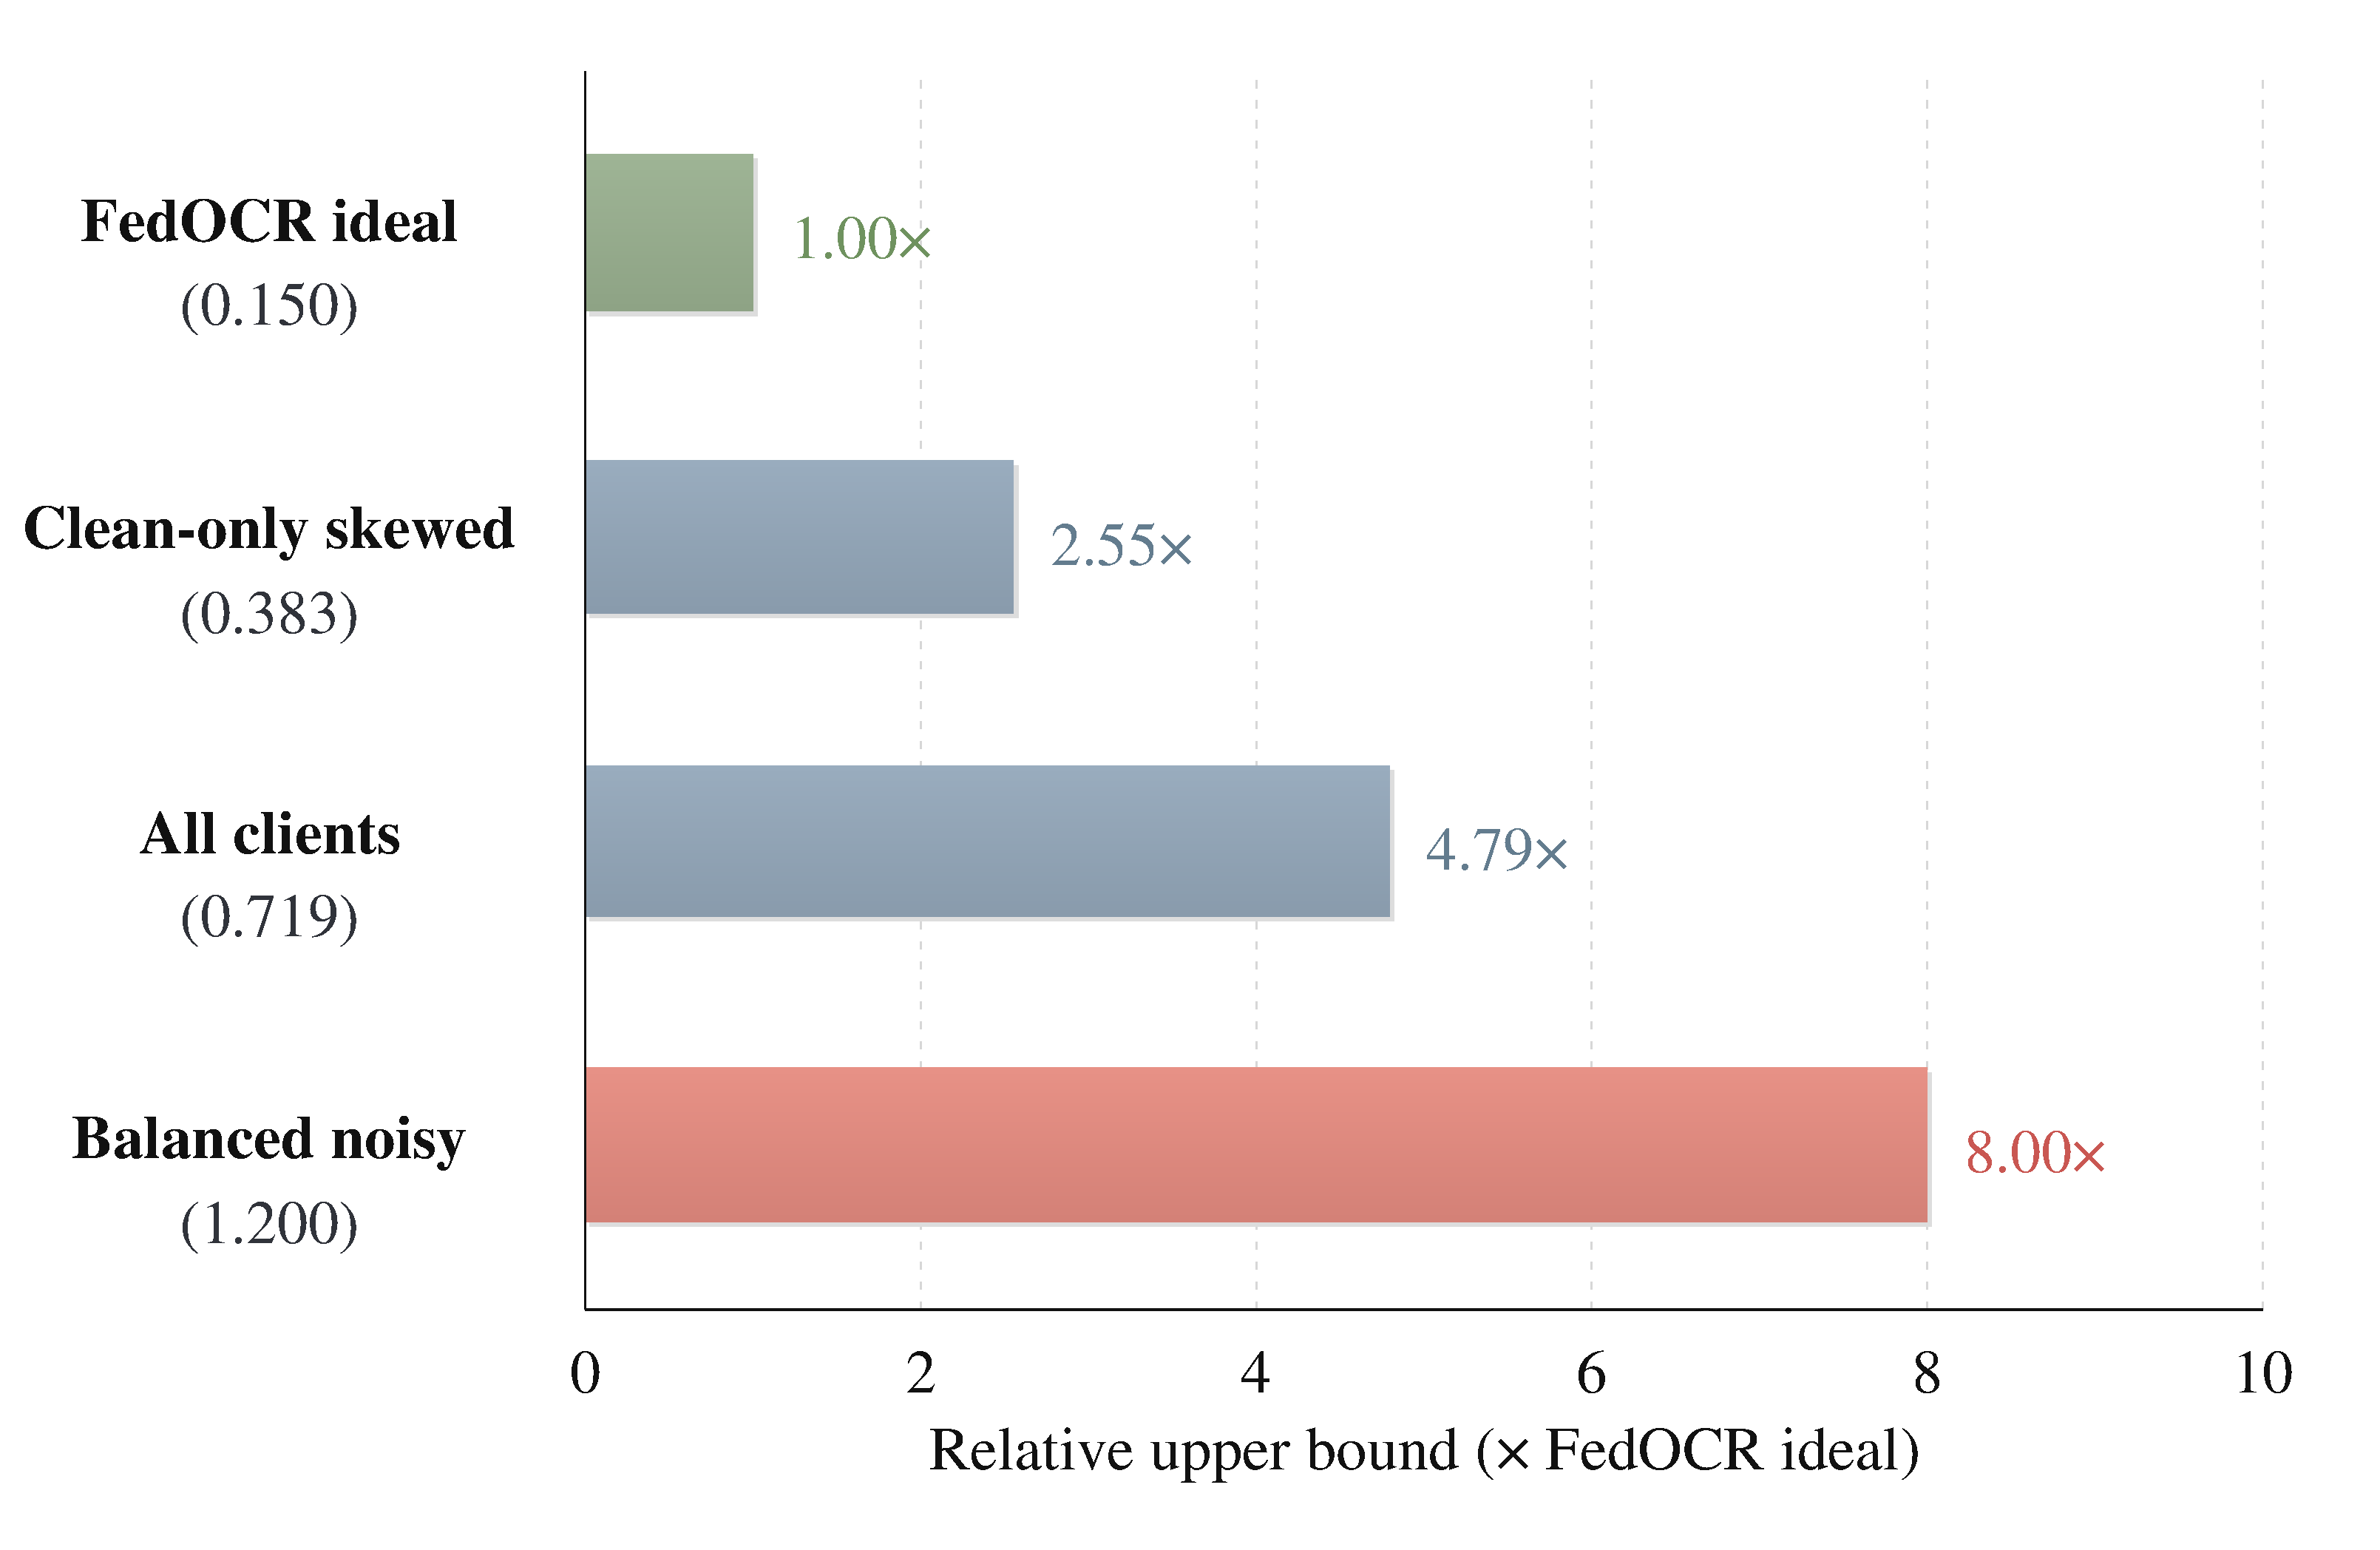
\includegraphics[width=0.30\textwidth]{figure/oracle/theoretical_bound.pdf}
    \hfill
    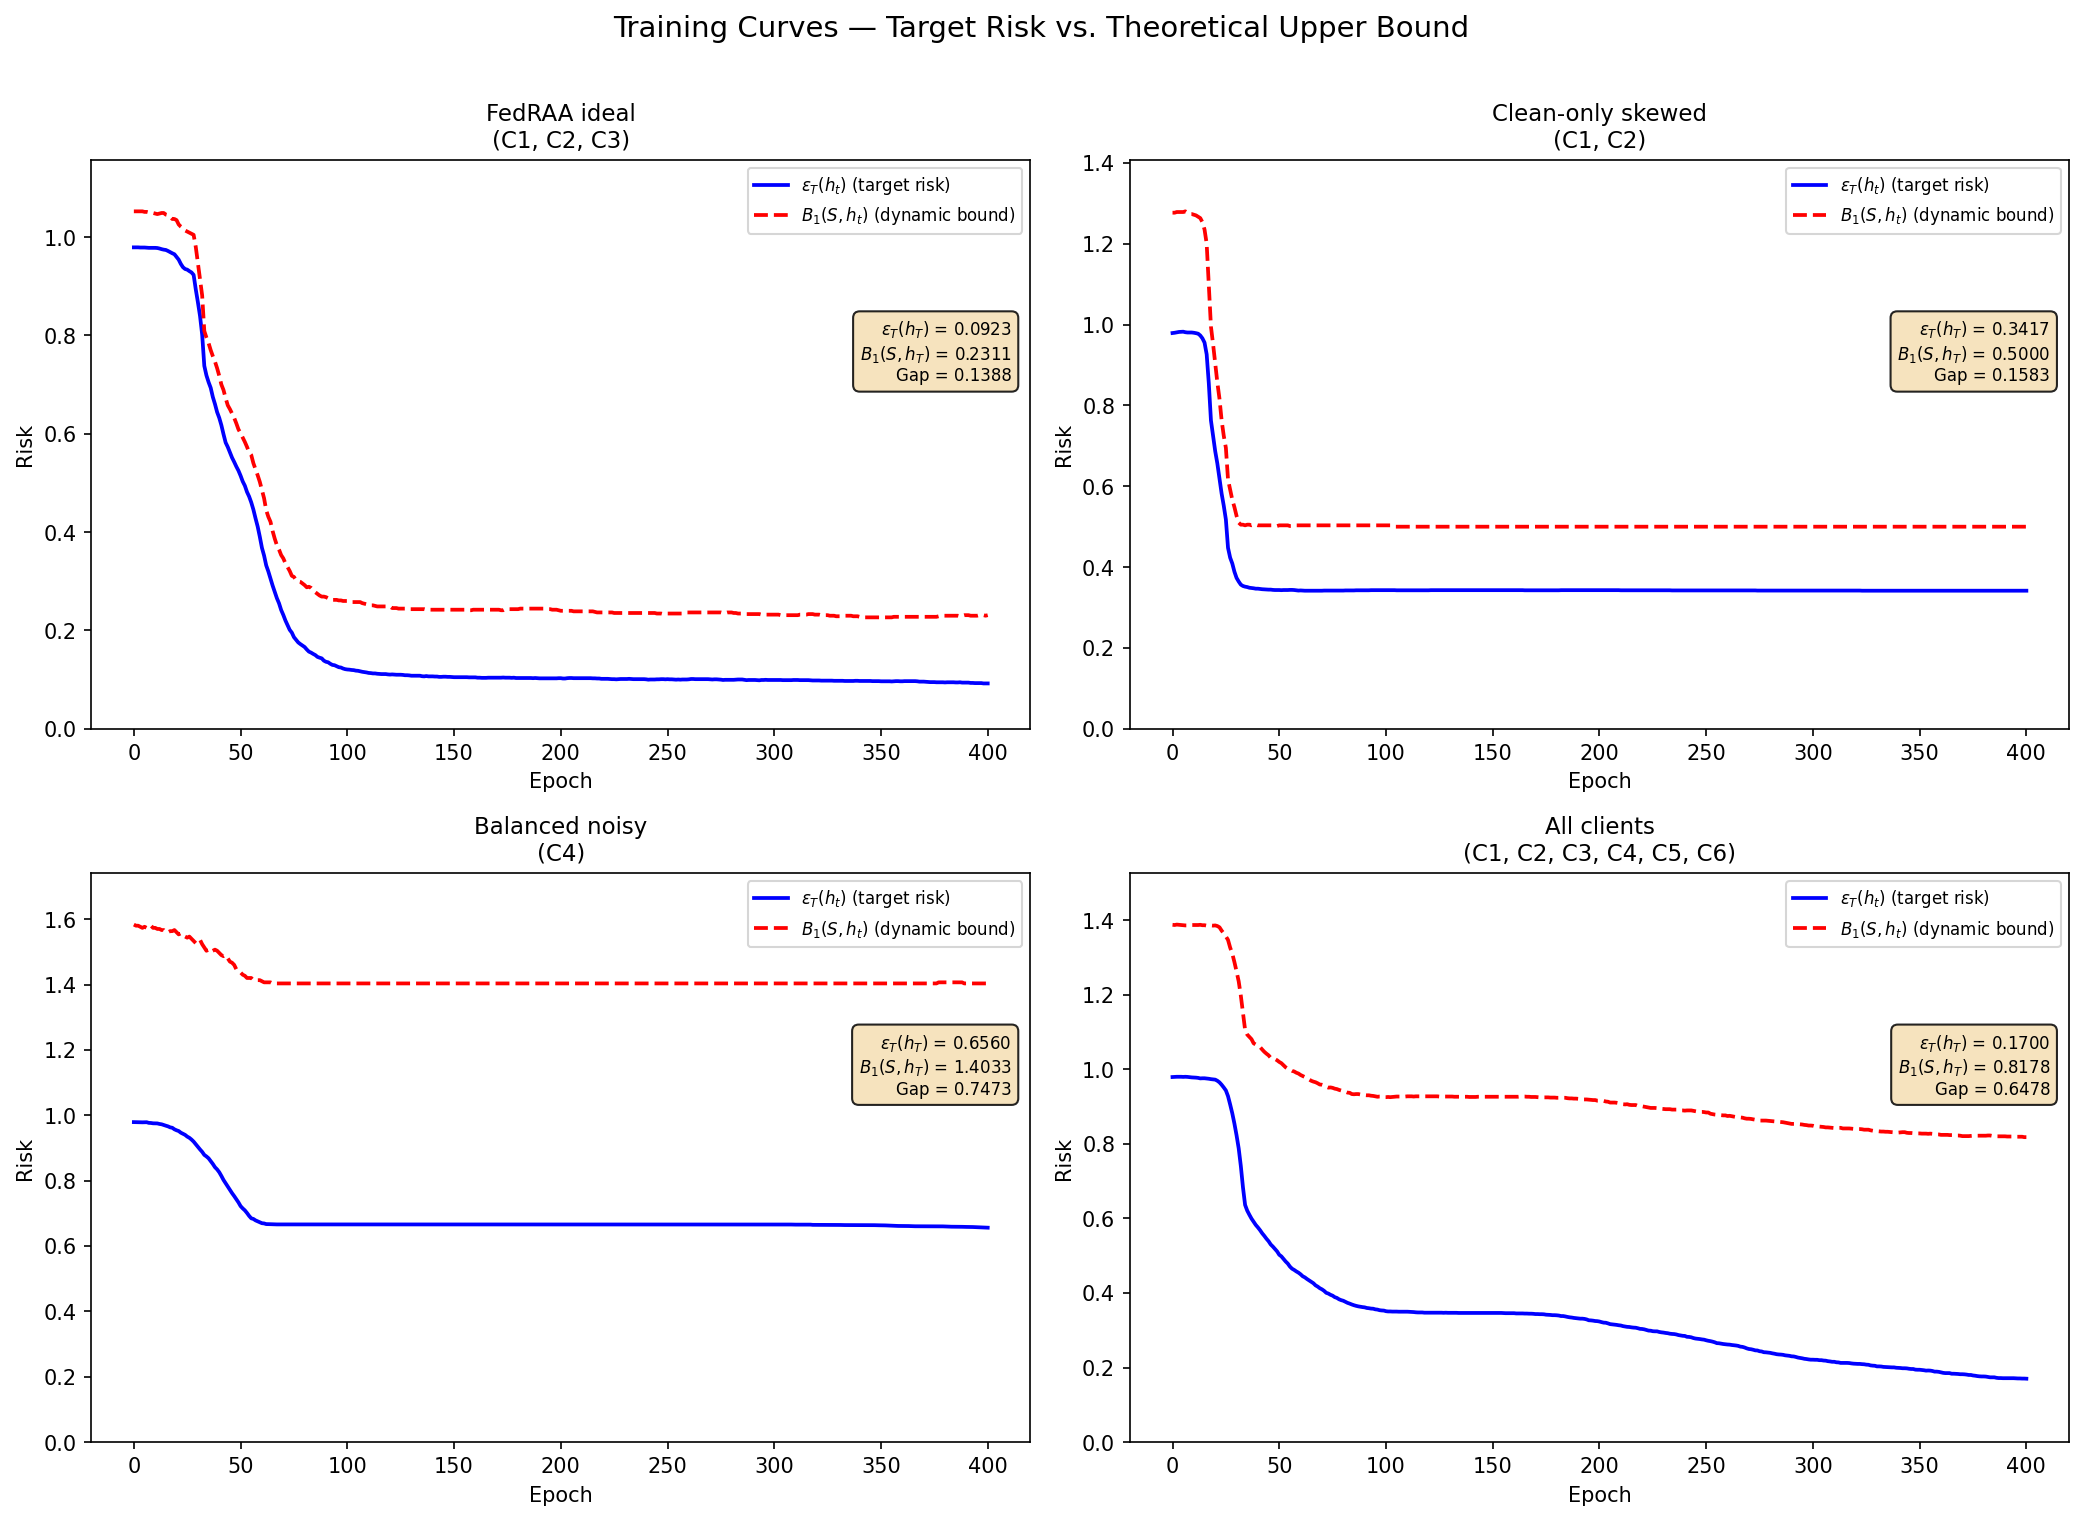
\includegraphics[width=0.36\textwidth]{figure/oracle/risk_bound.png}
    \hfill
    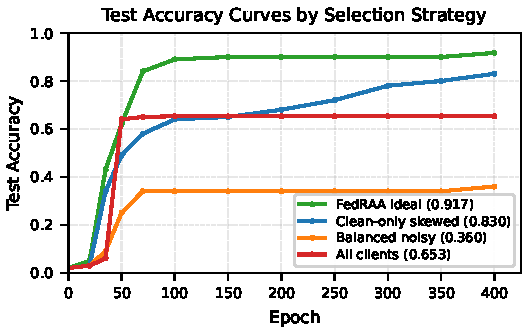
\includegraphics[width=0.30\textwidth]{figure/oracle/acc.pdf}
    \caption{Oracle validation of the admission principle. Left: theoretical risk bound under different admission strategies. Middle: empirical target risk and theoretical upper bound during training. Right: test accuracy curves under the same oracle strategies. The FedRAA ideal subset jointly reduces label-noise risk and distribution mismatch, resulting in the smallest bound and the best empirical performance.}
    \label{fig:oracle_summary}
\end{figure*}

\subsection{Main experiments}
\label{subsec:exp_setup}
In this subsection, we evaluate whether FedRAA provides a useful pre-training admission rule rather than behaving as a random client filter. 
We consider two comparison groups.
The first group contains noisy-label FL methods: full-round robust training baselines RFA~\cite{pillutla2022robust}, FedGreed~\cite{kritharakis2025fedgreed}, LASA~\cite{xu2025lasa}, FedNed~\cite{lu2024fedned}, and FedNoRo~\cite{wu2023fednoro}, together with training-stage correction methods FedCorr~\cite{xu2022fedcorr}, FedCS~\cite{hao2025fedcs}, FedFixer~\cite{ji2024fedfixer}, and FedDiv~\cite{li2024feddiv}.
The second group contains client selection baselines: full participation (All), random selection (RS), distribution-aware selection (EMD and GS~\cite{ma2021client}), and optimization-driven selection (PoC~\cite{cho2022power} and FedCor~\cite{tang2022fedcor}).

\paragraph{Implementation details.}
Unless otherwise specified, the training data are split over $N=50$ clients and $K=20$ clients participate in each federated training run.
We use Dirichlet partitioning with concentration parameter $\alpha=0.5$ and a step-imbalance ratio of 5 to simulate Non-IID data.
Label noise is applied symmetrically at the client level.
The main experiments use linear and Gaussian heterogeneous noise; additional 2-phase and 3-phase noise settings are described in Appendix~\ref{app:noise_mode}.
All methods are trained for $T=200$ global rounds under the same maximum round budget.
For local training, we use Adam with learning rate $1\times10^{-4}$ and batch size 64 for CIFAR-10/100 and 16 for TinyImageNet.
\paragraph{Comparison with noisy-label FL}
\label{para:comp_nfl}
We first compare FedRAA with noisy-label FL baselines under linear and Gaussian heterogeneous noise.
Table~\ref{tab:noisy_fl_accuracy} reports the collected accuracy results on MedMNIST, CIFAR-10, and CIFAR-100.
In this comparison, FedRAA uses its proposed variable-size admission rule and automatically determines the number of admitted clients before training.
FedNoRo obtains the highest final accuracy in several full-round settings, especially on CIFAR-10 Gaussian noise and CIFAR-100.
FedRAA remains competitive while using an admission rule that trains only the selected client pool, and it still obtains second-best accuracy on both CIFAR-100 noise settings.
The MedMNIST columns make the dataset-dependent nature of final accuracy explicit: FedNoRo is strongest under linear noise, while LASA is strongest under Gaussian noise.
Therefore, the efficiency analysis below focuses on the cost required to reach matched target utility rather than claiming that FedRAA dominates every final-accuracy column.

\begin{table*}[t]
\centering
\caption{Test accuracy (\%) of representative noisy-label FL methods under heterogeneous label noise. Results are collected at $\alpha=0.5$ with 50 candidate clients and reported as mean$\pm$standard deviation. FedRAA uses the proposed automatic client-admission rule in this table. Best results are highlighted in bold and second-best results are underlined.}
\label{tab:noisy_fl_accuracy}
\setlength{\tabcolsep}{3.2pt}
\renewcommand{\arraystretch}{1.15}
\begin{tabular}{lcccccc}
\toprule
\multirow{2}{*}{\textbf{Method}} 
& \multicolumn{2}{c}{\textbf{MedMNIST}} 
& \multicolumn{2}{c}{\textbf{CIFAR-10}} 
& \multicolumn{2}{c}{\textbf{CIFAR-100}} \\
\cmidrule(lr){2-3} \cmidrule(lr){4-5} \cmidrule(lr){6-7}
& \textbf{Linear} & \textbf{Gaussian} & \textbf{Linear} & \textbf{Gaussian} & \textbf{Linear} & \textbf{Gaussian} \\
\midrule

All & 60.89$\pm$1.89 & 85.53$\pm$0.73 & 39.16$\pm$0.31 & 54.38$\pm$0.37 & 24.11$\pm$0.13 & 31.21$\pm$0.23 \\
\midrule
\multicolumn{7}{l}{\textit{Full-round robust training baselines}} \\
RFA~\cite{pillutla2022robust} & 63.38$\pm$3.24 & 83.05$\pm$0.67 & 35.52$\pm$0.10 & 47.68$\pm$0.45 & 20.52$\pm$0.07 & 30.31$\pm$0.23 \\
FedGreed~\cite{kritharakis2025fedgreed} & \underline{83.09$\pm$3.17} & 82.22$\pm$3.67 & \textbf{56.30$\pm$1.78} & 54.24$\pm$1.68 & 20.79$\pm$1.05 & 32.18$\pm$0.86 \\
LASA~\cite{xu2025lasa} & 54.97$\pm$0.51 & \textbf{87.52$\pm$0.57} & 42.97$\pm$0.23 & 56.20$\pm$0.31 & 23.69$\pm$0.15 & 31.03$\pm$0.12 \\
FedNed~\cite{lu2024fedned} & 64.29$\pm$0.54 & 86.52$\pm$0.58 & 39.72$\pm$0.09 & 55.41$\pm$0.30 & 23.63$\pm$0.04 & 32.73$\pm$0.11 \\
FedNoRo~\cite{wu2023fednoro} & \textbf{85.48$\pm$0.41} & \underline{87.22$\pm$0.42} & 51.14$\pm$0.21 & \textbf{61.09$\pm$0.34} & \textbf{30.20$\pm$0.09} & \textbf{38.28$\pm$0.16} \\
\midrule
\multicolumn{7}{l}{\textit{Training-stage correction baselines}} \\
FedCorr~\cite{xu2022fedcorr} & 55.54$\pm$13.10 & 85.18$\pm$1.02 & \underline{53.39$\pm$0.33} & 49.59$\pm$0.77 & 26.19$\pm$0.17 & 30.67$\pm$0.28 \\
FedCS~\cite{hao2025fedcs} & 56.60$\pm$3.02 & 79.12$\pm$0.76 & 31.77$\pm$0.48 & 47.43$\pm$0.25 & 19.84$\pm$0.33 & 23.46$\pm$0.18 \\
FedFixer~\cite{ji2024fedfixer} & 61.06$\pm$1.92 & 85.70$\pm$0.76 & 33.53$\pm$0.39 & 54.61$\pm$0.42 & 23.45$\pm$0.17 & 32.71$\pm$0.25 \\
FedDiv~\cite{li2024feddiv} & 60.75$\pm$1.91 & 85.39$\pm$0.75 & 41.84$\pm$0.74 & 54.49$\pm$0.16 & 22.53$\pm$0.51 & 31.40$\pm$0.12 \\
\midrule
FedRAA (ours) & 81.05$\pm$0.80 & 85.71$\pm$0.37 & 53.38$\pm$1.20 & \underline{58.68$\pm$1.81} & \underline{28.73$\pm$0.75} & \underline{33.17$\pm$0.84} \\
\bottomrule
\end{tabular}
\end{table*}

Table~\ref{tab:efficiency_linear} further summarizes the cost saving obtained by FedRAA at matched target accuracy.
For each scenario, the reference baseline is a strong non-FedRAA method in Table~\ref{tab:noisy_fl_accuracy} that reaches the target.
FedRAA reduces both computation and communication in all four matched-utility comparisons, with particularly large savings on CIFAR-10 and MedMNIST Gaussian noise.
This supports the main design goal of FedRAA: it is not merely another accuracy-oriented correction method, but a cost-efficient admission mechanism that avoids repeated training on unreliable clients.

\begin{table*}[!t]
\centering
\caption{FedRAA cost saving at matched target accuracy. For each scenario, the reference method is a strong non-FedRAA method in Table~\ref{tab:noisy_fl_accuracy} that reaches the target. Computation is reported in $10^6$ FEP and communication in GB. Saving is reported as computation / communication reduction relative to the reference method.}
\label{tab:efficiency_linear}
\setlength{\tabcolsep}{4.5pt}
\renewcommand{\arraystretch}{1.12}
\begin{tabular}{llcccc}
\toprule
\textbf{Scenario} & \textbf{Method} & \textbf{Target} & \textbf{Comp.} & \textbf{Comm.} & \textbf{Saving} \\
\midrule
\multirow{2}{*}{CIFAR-10 Linear} & FedGreed~\cite{kritharakis2025fedgreed} & \multirow{2}{*}{50\%} & 8.49 & 33.33 & -- \\
& FedRAA (ours) & & \textbf{3.08} & \textbf{11.17} & \textbf{63.7\% / 66.5\%} \\
\midrule
\multirow{2}{*}{CIFAR-10 Gaussian} & LASA~\cite{xu2025lasa} & \multirow{2}{*}{55\%} & 21.23 & 83.32 & -- \\
& FedRAA (ours) & & \textbf{4.47} & \textbf{18.33} & \textbf{79.0\% / 78.0\%} \\
\midrule
\multirow{2}{*}{MedMNIST Linear} & FedGreed~\cite{kritharakis2025fedgreed} & \multirow{2}{*}{80\%} & 1.17 & 20.83 & -- \\
& FedRAA (ours) & & \textbf{1.04} & \textbf{14.66} & \textbf{11.1\% / 29.6\%} \\
\midrule
\multirow{2}{*}{MedMNIST Gaussian} & LASA~\cite{xu2025lasa} & \multirow{2}{*}{85\%} & 3.75 & 66.65 & -- \\
& FedRAA (ours) & & \textbf{1.78} & \textbf{26.16} & \textbf{52.5\% / 60.8\%} \\
\bottomrule
\end{tabular}
\end{table*}

We also test whether the conclusion changes with the strength of Non-IID partitioning.
Table~\ref{tab:noniid_robustness} reports the collected CIFAR-100 results under linear noise for $\alpha\in\{0.1,0.5,1.0\}$.
FedRAA consistently improves over full participation by $3.28$--$4.62$ percentage points and remains competitive across all three heterogeneity levels, while FedNoRo achieves the strongest final accuracy in this full-round comparison.
These results show that the proposed admission rule remains effective across different degrees of data heterogeneity.

\begin{table}[H]
\centering
\caption{CIFAR-100 accuracy (\%) under linear noise with different Dirichlet Non-IID levels. Results are reported as mean$\pm$standard deviation. Best results are highlighted in bold and second-best results are underlined.}
\label{tab:noniid_robustness}
\setlength{\tabcolsep}{4pt}
\renewcommand{\arraystretch}{1.12}
\begin{tabular}{lccc}
\toprule
\textbf{Method} & $\alpha=0.1$ & $\alpha=0.5$ & $\alpha=1.0$ \\
\midrule
All & 18.39$\pm$0.15 & 24.11$\pm$0.15 & 24.17$\pm$0.23 \\
RFA~\cite{pillutla2022robust} & 17.32$\pm$0.17 & 20.52$\pm$0.05 & 21.31$\pm$0.20 \\
FedGreed~\cite{kritharakis2025fedgreed} & 8.73$\pm$1.45 & 20.79$\pm$1.05 & \underline{29.03$\pm$0.85} \\
LASA~\cite{xu2025lasa} & 17.63$\pm$0.11 & 23.69$\pm$0.17 & 25.44$\pm$0.23 \\
FedNed~\cite{lu2024fedned} & 17.57$\pm$0.26 & 23.63$\pm$0.03 & 24.06$\pm$0.20 \\
FedNoRo~\cite{wu2023fednoro} & \textbf{22.56$\pm$0.20} & \textbf{30.20$\pm$0.08} & \textbf{32.82$\pm$3.79} \\
FedCorr~\cite{xu2022fedcorr} & \underline{22.03$\pm$1.01} & 26.19$\pm$0.16 & 24.03$\pm$0.24 \\
FedCS~\cite{hao2025fedcs} & 14.07$\pm$0.26 & 19.84$\pm$0.20 & 21.43$\pm$0.80 \\
FedFixer~\cite{ji2024fedfixer} & 18.66$\pm$0.14 & 23.45$\pm$0.26 & 25.37$\pm$0.23 \\
FedDiv~\cite{li2024feddiv} & 17.73$\pm$0.13 & 22.53$\pm$0.30 & 23.88$\pm$0.21 \\
\midrule
FedRAA (ours) & 21.67$\pm$0.27 & \underline{28.73$\pm$0.72} & 28.93$\pm$0.52 \\
\bottomrule
\end{tabular}
\end{table}


\paragraph{Comparison with client selection}
\label{para:comp_cs}
We compare FedRAA with multiple baselines under different label-noise levels to validate the effectiveness of the proposed method. For a fair comparison with existing client-selection methods, Table~\ref{tab:selection_merged} fixes the participation budget for all methods, including FedRAA, so that 20 out of 50 clients are selected to participate in federated training. This differs from Table~\ref{tab:noisy_fl_accuracy}, where FedRAA uses its automatic variable-size admission rule.

Figure~\ref{fig:triple_figures} illustrates the convergence behavior under the linear heterogeneous noise setting, while additional curves are provided in Appendix~\ref{app:more_curves}. Compared with the baselines, FedRAA exhibits faster convergence and more stable training dynamics, especially under high-noise conditions where other methods suffer from noticeable fluctuations or performance degradation. This indicates that FedRAA can effectively mitigate the adverse impact of noisy or biased clients during the optimization process.
Table~\ref{tab:selection_merged} further reports the final test accuracy across all datasets and noise patterns. FedRAA consistently achieves the best or near-best performance in most settings, demonstrating that its advantage generalizes across different noise configurations rather than relying on a specific corruption pattern.

Taken together, the convergence behavior and final performance jointly demonstrate the effectiveness of the proposed client selection strategy. FedRAA is able to admit clients that provide more reliable and informative updates while excluding those with noisy or biased data, leading to both stable optimization and improved generalization. In contrast, loss-driven or distribution-only baselines are more sensitive to heterogeneous noise, either over-selecting high-loss noisy clients or preserving distributional coverage at the cost of admitting corrupted participants.

\begin{table*}[!t]
\centering
\caption{Test accuracy (\%) of client selection methods under three heterogeneous noise settings. For fair client-selection comparison, all methods, including FedRAA, select a fixed budget of 20 clients. Results are reported as mean$\pm$standard deviation over the converged stage. Best results are highlighted in bold, and second-best results are underlined.}
\label{tab:selection_merged}
\setlength{\tabcolsep}{2.2pt}
\renewcommand{\arraystretch}{1.10}
\scriptsize
\begin{tabular*}{\textwidth}{@{\extracolsep{\fill}}lccccccccc@{}}
\toprule
\multirow{2}{*}{Method}
& \multicolumn{3}{c}{CIFAR-10}
& \multicolumn{3}{c}{CIFAR-100}
& \multicolumn{3}{c}{Tiny-ImageNet} \\
\cmidrule(lr){2-4}\cmidrule(lr){5-7}\cmidrule(lr){8-10}
& Linear & 2-Ph. & 3-Ph.
& Linear & 2-Ph. & 3-Ph.
& Linear & 2-Ph. & 3-Ph. \\
\midrule
PoC\cite{cho2022power}
& 14.79$\pm$0.29 & 43.68$\pm$0.33 & 66.46$\pm$0.21
& 5.46$\pm$0.21 & 25.12$\pm$0.23 & 36.40$\pm$0.12
& 2.91$\pm$0.11 & 23.36$\pm$0.12 & 36.05$\pm$0.12 \\

RS
& 39.31$\pm$0.36 & \underline{66.00$\pm$0.22} & \underline{72.25$\pm$0.50}
& 23.10$\pm$0.14 & \underline{36.46$\pm$0.44} & 36.40$\pm$0.11
& 19.52$\pm$0.09 & \underline{33.60$\pm$0.09} & \underline{37.62$\pm$0.19} \\

EMD
& 31.97$\pm$0.30 & 62.78$\pm$0.57 & 71.82$\pm$0.27
& 22.20$\pm$0.32 & 32.55$\pm$0.14 & 37.42$\pm$0.16
& 21.76$\pm$0.20 & 31.89$\pm$0.17 & 37.42$\pm$0.16 \\

GS\cite{ma2021client}
& \underline{46.88$\pm$0.45} & 63.28$\pm$0.37 & 63.02$\pm$0.29
& \underline{26.95$\pm$0.14} & 34.30$\pm$0.34 & \underline{37.64$\pm$0.21}
& \underline{24.88$\pm$0.09} & 31.86$\pm$0.29 & 37.31$\pm$0.21 \\

FedCor\cite{tang2022fedcor}
& 38.22$\pm$2.06 & 63.69$\pm$0.47 & 64.64$\pm$0.19
& 16.50$\pm$0.16 & 38.10$\pm$0.34 & 38.20$\pm$0.23
& 21.89$\pm$0.23 & 30.50$\pm$0.21 & 34.40$\pm$0.31 \\
\midrule
FedRAA(ours)
& \textbf{56.20$\pm$0.13} & \textbf{74.93$\pm$0.28} & \textbf{76.12$\pm$0.22}
& \textbf{30.71$\pm$0.12} & \textbf{39.11$\pm$0.23} & \textbf{40.57$\pm$0.18}
& \textbf{27.88$\pm$0.15} & \textbf{36.46$\pm$0.17} & \textbf{38.16$\pm$0.17} \\
\bottomrule
\end{tabular*}
\end{table*}

\paragraph{Hyperparameter sensitivity}
We study three key hyperparameters in the admission stage: the noise-adaptive strength, the first-round local epoch budget used to compute admission indicators, and the threshold range $\eta$.
Figure~\ref{fig:hyperparameter_sensitivity} reports the sensitivity results on the CIFAR-10 linear-noise setting.
The three sweeps show that FedRAA is sensitive to overly conservative or overly permissive admission, but a moderate setting consistently balances reliability and coverage.

\begin{figure*}[t]
    \centering
    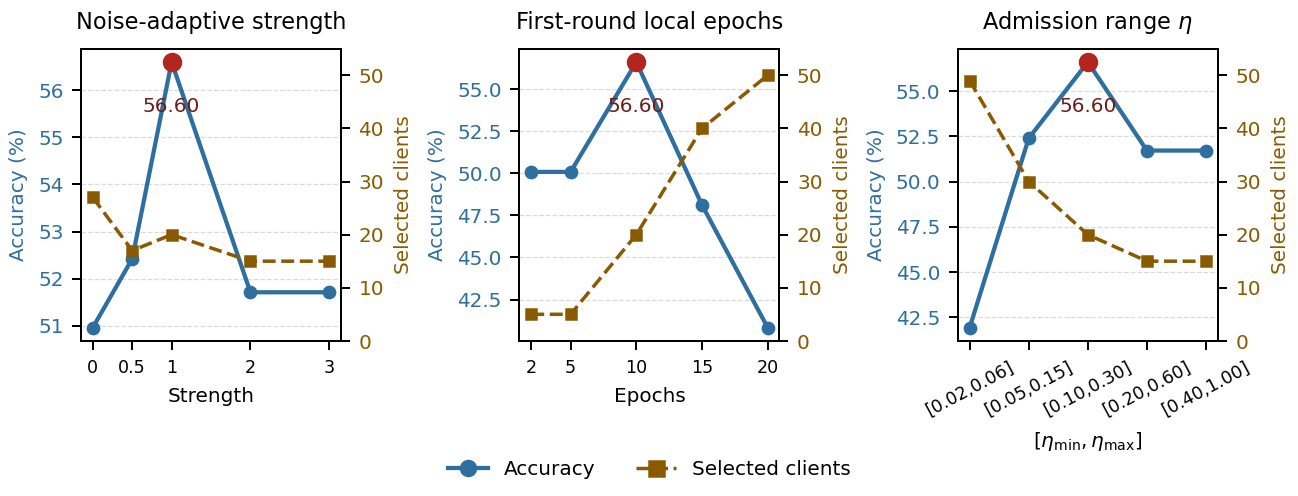
\includegraphics[width=0.85\textwidth]{figure/hyperparameter_sensitivity.png}
    \caption{Hyperparameter sensitivity on CIFAR-10 under linear heterogeneous noise. Each panel reports the test accuracy and the number of selected clients when varying one admission-stage hyperparameter while keeping the others fixed.}
    \label{fig:hyperparameter_sensitivity}
\end{figure*}

For the strength coefficient, setting the value to zero admits too many clients, while overly large values shrink the pool and reduce accuracy.
The best result is obtained at strength $=1$, suggesting that reliability and representativeness should be balanced rather than dominated by either side.
For the first-round epoch budget, too few epochs produce weak admission indicators and select only five clients, whereas too many epochs make the indicators overly permissive and eventually recover almost full participation.
The best budget is 10 epochs.
For $\eta$, a small threshold range admits many noisy clients, while a large range becomes too strict.
The default range $[0.10,0.30]$ selects 20 clients and achieves the best accuracy, which we use in the main experiments.
Additional client-pool-size curves are provided in Appendix Fig.~\ref{fig:screening}.

\paragraph{Compatibility with training-stage noise correction}
We further evaluate whether FedRAA can be combined with Co-teach+\cite{yu2019coteachingplus}, a training-stage noisy-label correction method. 
As shown in Table~\ref{tab:coteach_merged}, FedRAA and Co-teach+ are complementary: combining them improves performance in most settings. 
This suggests that pre-training client admission and training-stage label correction address different sources of robustness.
\subsection{Analysis of Selected Client Subsets}
\label{subsec:subset_analysis}

To understand why FedRAA improves robustness, we analyze the clean/noisy class composition of the selected clients. 
Figure~\ref{fig:subset_composition_main} reports the class-wise composition of the selected subsets under linear heterogeneous noise. 
FedRAA selects a subset with more clean samples and fewer noisy samples across most classes, while maintaining more balanced class coverage. 
In contrast, competing methods either accumulate more noisy samples or fail to cover clean samples in certain classes. 
This confirms that FedRAA improves both reliability and representativeness at the client-subset level.

\begin{figure}[t]
    \centering
    
\includegraphics[width=0.48\linewidth]{figure/数据分布/线性加噪/cifar10.png}
    
\includegraphics[width=0.48\linewidth]{figure/数据分布/线性加噪/cifar100.png}
    \caption{Class-wise clean/noisy sample composition of selected client subsets under linear heterogeneous noise. Positive bars denote clean samples, while negative bars denote noisy samples.}
    \label{fig:subset_composition_main}
\end{figure}

\begin{table}[t]
\centering
\caption{Ablation study on CIFAR-10 under linear heterogeneous noise. The table isolates the effect of reliability scoring, representativeness scoring, and noise-adaptive calibration.}
\label{tab:ablation_fedraa}
\setlength{\tabcolsep}{5pt}
\renewcommand{\arraystretch}{1.15}
\begin{tabular}{lcccc}
\toprule
\textbf{Variant} 
& \textbf{Reliab.} 
& \textbf{Represent.} 
& \textbf{Adaptive} 
& \textbf{Test Acc. (\%)} \\
\midrule

Random selection     & -- & -- & -- & 39.81$\pm$0.32 \\
All clients          & -- & -- & -- & 39.67$\pm$0.33 \\
Reliability only     & \checkmark & $\times$ & $\times$ & \underline{55.60$\pm$0.30} \\
Represent. only      & $\times$ & \checkmark & $\times$ & 30.69$\pm$0.52 \\
w/o adaptive calib.  & \checkmark & \checkmark & $\times$ & 53.22$\pm$0.16 \\
\midrule
FedRAA               & \checkmark & \checkmark & \checkmark & \textbf{56.60$\pm$0.29} \\

\bottomrule
\end{tabular}
\end{table}


\subsection{Ablation Study}
\label{subsec:ablation}

We ablate the two scoring terms and the adaptive calibration mechanism.
Table~\ref{tab:ablation_fedraa} shows that reliability is the dominant factor under severe heterogeneous noise: using the reliability score alone improves accuracy from $39.81\%$ to $55.60\%$.
Using the distribution score alone performs poorly, which indicates that distributional coverage cannot compensate for heavily corrupted local supervision.
The full FedRAA model further improves over the non-adaptive variant by $3.38$ percentage points, confirming that the noise-adaptive calibration helps balance reliability and representativeness instead of relying on a fixed weighting rule.

\section{Discussion}

FedRAA relies on proxy-based evidence because the server cannot inspect clients' raw data under the privacy constraints of FL.
This design makes the method practical for pre-training admission, but it also means that the quality of the proxy set affects the reliability of both admission signals.
Predictive entropy should therefore be interpreted as a proxy for client-side predictive unreliability rather than as a direct estimator of the true label-noise rate.
Similarly, the KL-based representativeness term measures alignment with the server-held proxy distribution, so a biased or outdated proxy set may shift the admitted pool toward the wrong target prior.
In long-running deployments where client populations or target distributions evolve, the one-shot admission rule may also need to be combined with periodic proxy refresh or lightweight re-admission.
These limitations do not change the main conclusion, but they clarify the conditions under which proactive client admission is most useful.

\section{Conclusion}

This paper studies robust federated learning from the perspective of pre-training client admission.
Under coupled label noise and Non-IID heterogeneity, simply admitting more clients can introduce unreliable supervision and target-mismatched updates, while selecting only clean clients may sacrifice distributional coverage.
To address this trade-off, we propose FedRAA, a reliability- and representativeness-aware admission framework that constructs a client subset before federated optimization begins.
FedRAA estimates client reliability through proxy-set predictive entropy and measures subset-level representativeness through KL-based proxy distribution matching.
Our theoretical analysis connects these two proxy signals to label-noise contamination and target-distribution mismatch in a unified target-risk view.

Experiments across multiple datasets, noise patterns, and heterogeneity levels show that FedRAA selects lower-noise and more complementary client subsets, achieves competitive or superior robust accuracy, and reduces computation and communication cost at matched target accuracy.
The ablation results further confirm that reliability scoring is essential under severe heterogeneous noise, while representativeness and adaptive calibration improve the balance between clean supervision and coverage.
These findings suggest that robust FL should not only correct unreliable updates during training, but also proactively control the quality of the admitted participant pool.
Future work will explore adaptive proxy construction, privacy-preserving proxy refinement, and admission strategies that can be updated over long-running federated deployments.

\bibliographystyle{IEEEtran}
\bibliography{FedPeD_refs}

\appendices

\section{Existence of harmful risk-prone clients}
\label{app:harmful_risk_prone_client}
Let $S\subseteq\mathcal{C}$ be a currently admitted client subset and let 
$j\in\mathcal{C}\setminus S$ be an additional candidate client. 
Denote $S^+=S\cup\{j\}$. 
Suppose the target-risk upper bound for subset $S$ is written as
\[
\mathcal{B}(S)
=
\epsilon_S^n(h_S)
+
\xi_{\mathrm{noise}}(S)
+
\mathcal{D}(T||S).
\]
Define the data-benefit term of adding client $j$ as
\[
G_j(S)
=
\epsilon_S^n(h_S)
-
\epsilon_{S^+}^n(h_{S^+}),
\]
and define the risk-increase term as
\[
R_j(S)
=
\left[
\xi_{\mathrm{noise}}(S^+)-\xi_{\mathrm{noise}}(S)
\right]
+
\left[\mathcal{D}(T||S^+)
-
\mathcal{D}(T||S)\right].
\]
If
\[
R_j(S)>G_j(S),
\]
then
\[
\mathcal{B}(S^+)>\mathcal{B}(S).
\]
That is, admitting client $j$ worsens the target-risk upper bound.


\begin{proof}
By definition,
\[
\begin{aligned}
\mathcal{B}(S^+)-\mathcal{B}(S)
&=
\epsilon_{S^+}^n(h_{S^+})
-
\epsilon_S^n(h_S)
\\
&\quad+
\left[
\xi_{\mathrm{noise}}(S^+)-\xi_{\mathrm{noise}}(S)
\right]
\\
&\quad+
\left[\mathcal{D}(T||S^+)
-
\mathcal{D}(T||S)\right].
\\
&=
-G_j(S)+R_j(S).
\end{aligned}
\]
Therefore, if $R_j(S)>G_j(S)$, then 
$\mathcal{B}(S^+)-\mathcal{B}(S)>0$, which proves the claim.
\end{proof}

\section{Additional theoretical details}
\label{app:theory_appendix}
\subsection{Proof of Lemma~\ref{lem:noise_bridge}}
\begin{proof}
For any distribution $P$ over $(X,Y)$, the risk of $h$ is defined as
$\epsilon_P(h)=\mathbb E_{(X,Y)\sim P}[\ell(h(X),Y)]$.
Since $\mathcal Y=\{1,\dots,K\}$ is discrete, by the law of total expectation,
\begin{align}
\epsilon_P(h)
&=
\mathbb E_{X}
\left[
\mathbb E_{Y\mid X}
\left[
\ell(h(X),Y)
\mid X
\right]
\right] \\
&=
\mathbb E_{x\sim P_X}
\left[
\sum_{c=1}^{K}
P(Y=c\mid x)\ell(h(x),c)
\right].
\label{eq:risk_total_expectation}
\end{align}
Under Assumption~\ref{assump:label_only_noise}, $P_S^c(X,Y)$ and $P_S^n(X,\widetilde Y)$ share the same input marginal $P_S^X$.
Applying Eq.~\eqref{eq:risk_total_expectation} to the clean and noisy mixtures gives
\begin{align}
\epsilon_S^c(h)
&=
\mathbb{E}_{x\sim P_S^X}
\left[
\sum_{c=1}^{K}
P_S^c(Y=c\mid x)
\ell(h(x),c)
\right],\\
\epsilon_S^n(h)
&=
\mathbb{E}_{x\sim P_S^X}
\left[
\sum_{c=1}^{K}
P_S^n(\widetilde Y=c\mid x)
\ell(h(x),c)
\right].
\end{align}
Therefore,
\begin{align}
&\big|\epsilon_S^c(h)-\epsilon_S^n(h)\big|\\
&= \Bigg|
\mathbb{E}_{x\sim P_S^X} \sum_{c=1}^{K} 
\Big( P_S^c(Y=c\mid x) - P_S^n(\widetilde Y=c\mid x) \Big)
\ell(h(x),c)
\Bigg| \notag \\
&\le \mathbb{E}_{x\sim P_S^X} 
\sum_{c=1}^{K} 
\Big| P_S^c(Y=c\mid x) - P_S^n(\widetilde Y=c\mid x) \Big|
\cdot |\ell(h(x),c)| \notag \\
&\le \mathbb{E}_{x\sim P_S^X} 
\sum_{c=1}^{K} 
\Big| P_S^c(Y=c\mid x) - P_S^n(\widetilde Y=c\mid x) \Big| \notag \\
&= \xi_{\mathrm{noise}}(S)
\end{align}
The first inequality follows from the triangle inequality, and the second follows from the bounded-loss assumption $0\le \ell\le 1$.
\end{proof}

\subsection{Proof of Lemma~\ref{lem:label_shift_transfer}}
\begin{proof}
By the standard variational characterization of total variation distance~\cite{gibbs2002choosing}, for any measurable function $f$ with $0\le f\le 1$,
\[
\left|
\mathbb E_P[f]-\mathbb E_Q[f]
\right|
\le
\mathrm{TV}(P,Q).
\]
Applying this inequality to $f_h(x,y)=\ell(h(x),y)$ yields
\begin{align}
&\big|\epsilon_T(h)-\epsilon_S^c(h)\big| \\
&=
\left|
\mathbb{E}_{(x,y)\sim P_T}
\left[
\ell(h(x),y)
\right]
-
\mathbb{E}_{(x,y)\sim P_S^c}
\left[
\ell(h(x),y)
\right]
\right| \\
&\le
\mathrm{TV}(P_T,P_S^c).
\end{align}
Since the class-conditional distributions are shared,
\begin{equation}
\label{eq:TV_equality}
\mathrm{TV}(P_T,P_S^c)
=
\frac{1}{2}
\sum_{y=1}^{K}
\left|
q_T(y)-\bar q_S(y)
\right|
=
\frac{1}{2}
\|\bar q_S-q_T\|_1.
\end{equation}
Therefore,
\[
\epsilon_T(h)
\le
\epsilon_S^c(h)
+
\frac{1}{2}\|\bar q_S-q_T\|_1.
\]
\end{proof}
\subsection{Proof of Theorem~\ref{thm:residualized_proxy_bound}}
\begin{proof}
By Theorem~\ref{thm:main_bound},
\begin{equation}
\epsilon_T(h)
\le
\epsilon_S^n(h)
+
\xi_{\mathrm{noise}}(S)
+
\frac12\|\bar q_S-q_T\|_1.
\end{equation}
By the definition of $r_H(S;c_H)$, we have
\begin{equation}
\xi_{\mathrm{noise}}(S)
\le
c_H\widehat{\xi}_{H}(S)
+
r_H(S;c_H).
\end{equation}
For the distribution mismatch term, the triangle inequality gives
\begin{align}
\frac12\|\bar q_S-q_T\|_1
&\le
\frac12\|\bar q_S-z_S\|_1
+
\frac12\|z_S-z_S^\epsilon\|_1
\\&+
\frac12\|z_S^\epsilon-p_{\mathrm{proxy}}\|_1
+
\frac12\|p_{\mathrm{proxy}}-q_T\|_1\\
&=
r_Z(S)
+
r_\epsilon(S)
+
\mathrm{TV}(z_S^\epsilon,p_{\mathrm{proxy}})
+
r_T.
\end{align}
By Pinsker's inequality, also known as the Csisz{\'a}r--Kullback--Pinsker inequality~\cite{pinsker1964information,csiszar1967information},
\begin{equation}
\mathrm{TV}(z_S^\epsilon,p_{\mathrm{proxy}})
\le
\sqrt{
\frac12
\mathrm{KL}
\left(
p_{\mathrm{proxy}}\|z_S^\epsilon
\right)
}.
\end{equation}
Combining the above inequalities gives Eq.~\eqref{eq:residualized_proxy_bound}.
\end{proof}
\subsection{Proof of Corollary~\ref{cor:proxy_consistency_surrogate}}
\begin{proof}
By Theorem~\ref{thm:residualized_proxy_bound},
\begin{align}
\epsilon_T(h)
&\le
\epsilon_S^n(h)
+
c_H\widehat{\xi}_{H}(S) \\
&
+
\sqrt{
\frac12
\mathrm{KL}
\left(
p_{\mathrm{proxy}}\|z_S^\epsilon
\right)
}
+
R_{\mathrm{proxy}}(S;c_H).
\end{align}
For any $x\ge0$ and $\lambda_s>0$, Young's inequality gives
$\sqrt{x/2}\le \lambda_s x + 1/(8\lambda_s)$.
Applying this inequality to $x=\mathrm{KL}(p_{\mathrm{proxy}}\|z_S^\epsilon)$ and using
$R_{\mathrm{proxy}}(S;c_H)\le\delta_{\mathrm{proxy}}$ gives Eq.~\eqref{eq:proxy_consistency_bound}.
\end{proof}
\subsection{Derivation of the Label-Prior TV Distance}
\label{app:tv_label_prior}

This appendix proves that, under the shared class-conditional assumption, the total variation distance between the target distribution and the selected clean client mixture reduces to the $\ell_1$ distance between their label priors.

Recall Assumption~\ref{assump:label_shift}. 
The target distribution and the selected clean client mixture are written as
\[
P_T(x,y)=p(x\mid y)q_T(y),
\qquad
P_S^c(x,y)=p(x\mid y)\bar q_S(y),
\]
where
\[
\bar q_S=\sum_{i\in S}w_i(S)q_i.
\]
Using the definition of total variation distance,
\begin{align}
&\mathrm{TV}(P_T,P_S^c)\\
&=
\frac{1}{2}
\sum_{y=1}^{K}
\int
\left|
P_T(x,y)-P_S^c(x,y)
\right|
dx \\
&=
\frac{1}{2}
\sum_{y=1}^{K}
\int
\left|
p(x\mid y)q_T(y)
-
p(x\mid y)\bar q_S(y)
\right|
dx \\
&=
\frac{1}{2}
\sum_{y=1}^{K}
\int
p(x\mid y)
\left|
q_T(y)-\bar q_S(y)
\right|
dx \\
&=
\frac{1}{2}
\sum_{y=1}^{K}
\left|
q_T(y)-\bar q_S(y)
\right|
\int p(x\mid y)dx.
\end{align}
Since $p(x\mid y)$ is a conditional distribution, $\int p(x\mid y)dx=1$ for every class $y$. 
Therefore,
\begin{equation}
\mathrm{TV}(P_T,P_S^c)
=
\frac{1}{2}
\sum_{y=1}^{K}
\left|
q_T(y)-\bar q_S(y)
\right|
=
\frac{1}{2}
\|\bar q_S-q_T\|_1.
\end{equation}

Thus, under shared class-conditional distributions, the source--target discrepancy is fully determined by the mismatch between the selected client label prior $\bar q_S$ and the target label prior $q_T$.

\subsection{Entropy as a proxy for client noise}
\label{app:entropy_proxy}

We now formalize why average predictive entropy is a useful reliability signal.

\begin{proposition}[Entropy--noise bridge]
\label{prop:entropy_bridge_appendix}
Fix client $i$ and assume $K$-class symmetric label noise with rate $\rho_i\in[0,1-1/K)$. Let
\begin{equation}
T_{\rho_i}
=
(1-\rho_i)I + \frac{\rho_i}{K-1}(\mathbf{1}\mathbf{1}^\top-I)
\end{equation}
be the noise transition matrix. For a proxy input $x$, denote the clean posterior by $\eta_i(x)\in\Delta^{K-1}$ and the noisy posterior by
\begin{equation}
\tilde \eta_i(x)=T_{\rho_i}\eta_i(x).
\end{equation}
Assume the proxy samples are $\delta_{\mathrm{sep}}$-separable in the sense that
\begin{equation}
\max_c \eta_i(c\mid x) \ge 1-\delta_{\mathrm{sep}},
\qquad \forall x\in\mathcal{D}_{\mathrm{proxy}},
\end{equation}
for some $\delta_{\mathrm{sep}}\in[0,1)$. Assume further that the local model predictions satisfy
\begin{equation}
\mathbb{E}_{x\sim P_{\mathrm{proxy}}}
\big[
\mathrm{KL}(\tilde\eta_i(x)\,\|\,p_i(\cdot\mid x))
\big]
\le \varepsilon_{\mathrm{cal}}.
\end{equation}
Define
\begin{equation}
 h_K(\rho)
 :=
 -(1-\rho)\log(1-\rho)
 - \rho\log\frac{\rho}{K-1}.
\end{equation}
Then the average predictive entropy
\begin{equation}
\bar H_i
:=
\mathbb{E}_{x\sim P_{\mathrm{proxy}}}
\big[H(p_i(\cdot\mid x))\big]
\end{equation}
obeys
\begin{equation}
\label{eq:entropy_bridge_appendix}
\bar H_i
\ge
(1-\delta_{\mathrm{sep}})h_K(\rho_i)
- \phi_K\!\left(\sqrt{\varepsilon_{\mathrm{cal}}/2}\right),
\end{equation}
where
\begin{align}
\phi_K(\delta)
&:=\delta\log(K-1)+h_2(\delta),\\
h_2(\delta)
&:=-\delta\log\delta-(1-\delta)\log(1-\delta).
\end{align}
Consequently, $\bar H_i$ is monotone increasing in $\rho_i$ up to a calibration- and separability-dependent relaxation.
\end{proposition}

\begin{proof}
Fix a proxy point $x$ and let $c^*(x):=\arg\max_c \eta_i(c\mid x)$. By separability, there exists a distribution $r_x\in\Delta^{K-1}$ such that
\begin{equation}
\eta_i(x)
=
(1-\delta_x)e_{c^*(x)} + \delta_x r_x,
\qquad 0\le \delta_x \le \delta_{\mathrm{sep}}.
\end{equation}
Applying the symmetric transition matrix gives
\begin{equation}
\tilde\eta_i(x)
=
(1-\delta_x)v_{\rho_i,c^*(x)} + \delta_x T_{\rho_i}r_x,
\end{equation}
where
\begin{equation}
v_{\rho_i,c^*}
:=
(1-\rho_i)e_{c^*}
+ \frac{\rho_i}{K-1}(\mathbf{1}-e_{c^*}).
\end{equation}
By concavity of entropy,
\begin{align}
H(\tilde\eta_i(x))
&\ge
(1-\delta_x)H\big(v_{\rho_i,c^*(x)}\big)
+\delta_x H\big(T_{\rho_i}r_x\big) \\
&\ge
(1-\delta_x)h_K(\rho_i)
\ge
(1-\delta_{\mathrm{sep}})h_K(\rho_i).
\end{align}
Now compare $p_i(\cdot\mid x)$ and $\tilde\eta_i(x)$. By Pinsker's inequality,
\begin{equation}
\|p_i(\cdot\mid x)-\tilde\eta_i(x)\|_1
\le
\sqrt{2\,\mathrm{KL}(\tilde\eta_i(x)\,\|\,p_i(\cdot\mid x))}.
\end{equation}
The Fannes--Audenaert continuity bound for entropy implies
\begin{equation}
\big|H(p_i(\cdot\mid x))-H(\tilde\eta_i(x))\big|
\le
\phi_K\!\left(\tfrac{1}{2}\|p_i(\cdot\mid x)-\tilde\eta_i(x)\|_1\right).
\end{equation}
Using Pinsker and Jensen,
\begin{equation}
\mathbb{E}_{x}\big[H(p_i(\cdot\mid x))\big]
\ge
\mathbb{E}_{x}\big[H(\tilde\eta_i(x))\big]
-
\phi_K\!\left(\sqrt{\varepsilon_{\mathrm{cal}}/2}\right).
\end{equation}
Combining with the lower bound on $H(\tilde\eta_i(x))$ yields \eqref{eq:entropy_bridge_appendix}. Finally, $h_K(\rho)$ is strictly increasing on $[0,1-1/K)$, so the ranking induced by $\bar H_i$ agrees with the ranking induced by $\rho_i$ up to the stated relaxation. \qed
\end{proof}

\paragraph{A useful corollary.}
Since $h_K$ is invertible on $[0,1-1/K)$, \eqref{eq:entropy_bridge_appendix} implies the conservative upper bound
\begin{equation}
\rho_i
\le
h_K^{-1}\!\left(
\frac{\bar H_i+\phi_K(\sqrt{\varepsilon_{\mathrm{cal}}/2})}{1-\delta_{\mathrm{sep}}}
\right).
\end{equation}
Under symmetric noise, this immediately yields
\begin{equation}
\xi_{\mathrm{noise}}(S)
\lesssim
2\sum_{i\in S}w_i(S)
\,h_K^{-1}\!\left(
\frac{\bar H_i+\phi_K(\sqrt{\varepsilon_{\mathrm{cal}}/2})}{1-\delta_{\mathrm{sep}}}
\right),
\end{equation}
which motivates the reliability score used in the main text.

\subsection{Combinatorial optimization and a submodular variant}
\label{app:submodular_variant}

The main algorithm uses a KL-based target-matching objective because it directly aligns the selected subset with the proxy target distribution. This objective is not guaranteed to be submodular. Nevertheless, the connection to classical subset selection can be made explicit via a closely related facility-location surrogate.

Let $\kappa(i,j)\ge 0$ be a similarity between the predictive signatures $z_i$ and $z_j$ defined in the main text. Consider the coverage function
\begin{equation}
G(S) := \sum_{j=1}^N \max_{i\in S} \kappa(i,j),
\end{equation}
and the set objective
\begin{equation}
F_{\mathrm{sub}}(S)
:=
\lambda_r\sum_{i\in S} r_i
+ \lambda_s G(S),
\qquad \lambda_r,\lambda_s\ge 0.
\end{equation}
The first term rewards reliable clients; the second term rewards representative coverage of the predictive-signature space.

\begin{proposition}[Submodular subset view]
\label{prop:submodular_appendix}
$F_{\mathrm{sub}}$ is monotone submodular. Consequently, maximizing $F_{\mathrm{sub}}(S)$ subject to $|S|\le M$ is NP-hard in general, and the classical greedy algorithm returns a subset $S_{\mathrm{greedy}}$ satisfying
\begin{equation}
F_{\mathrm{sub}}(S_{\mathrm{greedy}})
\ge
\left(1-\frac{1}{e}\right)
\max_{|S|\le M}F_{\mathrm{sub}}(S)
\end{equation}
\cite{nemhauser1978submodular,krause2014submodular}.
\end{proposition}

\begin{proof}
The modular term $\sum_{i\in S}r_i$ is monotone submodular because its marginal gain is constant. The facility-location term $G(S)$ is also monotone submodular: adding an element can only increase the pointwise maxima, and the marginal gain decreases as the current subset grows. A nonnegative linear combination of monotone submodular functions remains monotone submodular. The $(1-1/e)$ guarantee then follows from the classical theorem of Nemhauser \emph{et al.} \cite{nemhauser1978submodular}. \qed
\end{proof}

\paragraph{Interpretation.}
This proposition clarifies the conceptual role of FedRAA. The selected participant pool can be viewed as a \emph{robust client subset}: it compresses the candidate population into a smaller subset that preserves representative coverage while filtering out unreliable or outlying clients.

\section{Discussion on Proxy-Consistency Residuals}
\label{app:proxy_consistency}

This appendix discusses when the residual terms in the residualized proxy admission bound are expected to be small.
Recall that Theorem~\ref{thm:residualized_proxy_bound} separates the observable proxy objective from the approximation residual
\[
R_{\mathrm{proxy}}(S;c_H)
=
r_H(S;c_H)
+
r_Z(S)
+
r_T
+
r_\epsilon(S),
\]
where
\[
\begin{aligned}
r_H(S;c_H)
&=
\left[
\xi_{\mathrm{noise}}(S)
-
c_H\widehat{\xi}_{H}(S)
\right]_+,
\\
r_Z(S)
&=
\frac12\|\bar q_S-z_S\|_1,
\\
r_T
&=
\frac12\|p_{\mathrm{proxy}}-q_T\|_1,
\\
r_\epsilon(S)
&=
\frac12\|z_S-z_S^\epsilon\|_1.
\end{aligned}
\]
These residuals are not directly optimized by FedRAA.
They quantify the gap between the population quantities in Theorem~\ref{thm:main_bound} and the proxy statistics used by the algorithm.
The proxy bound should therefore be interpreted conditionally: when these residuals are small, optimizing the observable entropy--KL surrogate is aligned with reducing the target-risk upper bound.

\subsection{When is the entropy residual $r_H$ small?}
\label{app:entropy_residual}

The entropy residual
\[
r_H(S;c_H)
=
\left[
\xi_{\mathrm{noise}}(S)
-
c_H\widehat{\xi}_{H}(S)
\right]_+
\]
measures whether the entropy-based proxy underestimates the population label-noise discrepancy.
It is small when proxy predictive entropy is positively aligned with client-level predictive unreliability induced by corrupted supervision.

This condition is more plausible when the following factors hold.
First, the proxy set should be representative of the target decision regions, so that uncertainty on $\mathcal D_{\mathrm{proxy}}$ reflects the instability of a locally adapted client model on target-relevant inputs.
Second, the local adaptation step should be long enough for the client model $f_i$ to reflect the statistical quality of client $i$, but not so long that it overfits corrupted labels with overconfident predictions.
Third, the model should be reasonably calibrated on the proxy distribution, so that predictive entropy is meaningful as an uncertainty measure.
Under these conditions, clients with stronger label corruption tend to produce less stable or less confident predictions on the proxy set, leading to larger $\widetilde H_i$.

However, predictive entropy is not a noise-specific statistic.
A large entropy value can also arise from hard examples, feature shift, model underfitting, class imbalance, or proxy-client mismatch.
Conversely, a heavily corrupted client may become overconfident after local overfitting, producing low entropy despite poor label quality.
For this reason, FedRAA interprets entropy as a proxy-set predictive unreliability measure rather than a direct estimator of the true label-noise rate.
In our experiments, we empirically examine the relationship between client noise severity and proxy predictive entropy to support this proxy choice.

\subsection{When is the coverage residual $r_Z$ small?}
\label{app:coverage_residual}

The coverage residual
\[
r_Z(S)
=
\frac12\|\bar q_S-z_S\|_1
\]
measures the mismatch between the clean selected-client label prior $\bar q_S$ and the proxy-predicted mixture $z_S$.
This residual is small when the proxy-predicted signatures preserve the relative target-facing class coverage of the selected clients.

This condition does not require $z_S$ to exactly recover each client's private clean label prior.
Instead, it requires that the proxy predictions of the locally adapted client models provide a useful class-profile signal for how the admitted client pool behaves on target-relevant inputs.
The condition is more plausible when the proxy set covers the target classes, the adapted client models retain class-discriminative information from their local data, and the hard prediction signatures are not dominated by noise or underfitting.
The sample-size weighting in $z_S=\sum_{i\in S}\omega_i(S)\hat r_i$ also mirrors the mixture prior $\bar q_S=\sum_{i\in S}w_i(S)q_i$, which helps align the proxy mixture with the population mixture when the signatures are informative.

The residual can be large when client models are poorly adapted, when local label noise severely distorts decision boundaries, or when the proxy distribution is far from the regions where client models are informative.
It can also be large under strong feature shift, because a client may have a useful local class distribution but produce biased predictions on the proxy set.
Therefore, $z_S$ should be understood as a target-facing predictive coverage statistic rather than an exact estimator of private clean label priors.

\subsection{When is the target-prior residual $r_T$ small?}
\label{app:target_prior_residual}

The target-prior residual
\[
r_T
=
\frac12\|p_{\mathrm{proxy}}-q_T\|_1
\]
measures how well the empirical proxy label distribution approximates the target label prior.
It is small when the server-held proxy dataset is sampled from, or deliberately constructed to match, the target test distribution.
For example, in a balanced classification benchmark, a class-balanced proxy set yields a small $r_T$ when the target prior is also balanced.
In practical deployments, this residual can be reduced by curating the proxy set to reflect the expected deployment distribution.

This residual can be large if the proxy set is biased, outdated, too small, or mismatched with the target population.
In that case, the KL term $\mathrm{KL}(p_{\mathrm{proxy}}\|z_S^\epsilon)$ encourages matching the proxy prior rather than the true target prior.
Thus, the reliability of the representativeness surrogate depends on the quality of the proxy dataset.

\subsection{Effect of the smoothing residual $r_\epsilon$}
\label{app:smoothing_residual}

The smoothing residual
\[
r_\epsilon(S)
=
\frac12\|z_S-z_S^\epsilon\|_1
\]
is introduced only for numerical stability when computing the forward KL divergence.
Since
\[
z_S^\epsilon(c)
=
\frac{z_S(c)+\epsilon}{1+K\epsilon},
\qquad c=1,\dots,K,
\]
we have $z_S^\epsilon(c)>0$ for every class, which avoids zero-support problems in $\mathrm{KL}(p_{\mathrm{proxy}}\|z_S^\epsilon)$.
For small $\epsilon$, the perturbation from $z_S$ to $z_S^\epsilon$ is small.
Indeed,
\[
z_S^\epsilon-z_S
=
\frac{\epsilon\mathbf 1-K\epsilon z_S}{1+K\epsilon},
\]
and therefore
\[
\|z_S^\epsilon-z_S\|_1
\le
\frac{\epsilon\|\mathbf 1\|_1+K\epsilon\|z_S\|_1}{1+K\epsilon}
=
\frac{2K\epsilon}{1+K\epsilon}.
\]
Thus,
\[
r_\epsilon(S)
=
\frac12\|z_S-z_S^\epsilon\|_1
\le
\frac{K\epsilon}{1+K\epsilon}.
\]
When $\epsilon$ is small, this residual is negligible compared with the main proxy terms.

\subsection{Summary}
\label{app:proxy_consistency_summary}

The residualized bound separates two roles.
The observable part,
\[
c_H\widehat{\xi}_{H}(S)
+
\lambda_s\mathrm{KL}(p_{\mathrm{proxy}}\|z_S^\epsilon),
\]
is the quantity optimized by FedRAA.
The residual part,
\[
R_{\mathrm{proxy}}(S;c_H)
=
r_H(S;c_H)+r_Z(S)+r_T+r_\epsilon(S),
\]
measures how well the proxy statistics approximate the corresponding population quantities.
Therefore, the theoretical role of FedRAA is conditional rather than unconditional: if the proxy set is target-relevant and the adapted client models yield informative uncertainty and class-signature statistics, then minimizing the entropy--KL surrogate is aligned with reducing the target-risk upper bound.

\section{Oracle Experiment Details}
\label{app:oracle_experiment_details}
\begin{table}[t]
\centering
\caption{Configuration of the oracle experiment. The six clients differ in both class-prior distribution and label-noise rate. Clients C1--C3 are low-noise but individually class-skewed, while their union provides a balanced class distribution.}
\label{tab:oracle_setup}
\setlength{\tabcolsep}{4pt}
\renewcommand{\arraystretch}{1.15}
\begin{tabular}{l|l}
\toprule
\textbf{Item} & \textbf{Setting} \\
\midrule
Task type & Three-class non-IID classification \\
Feature dimension & 2 \\
Input distribution & Gaussian class-conditionals \\
Class means & $\mu_1=(-2,0),\ \mu_2=(2,0),\ \mu_3=(0,2)$ \\
Covariance & $\sigma=0.9$ \\
Target prior & $q_T=(1/3,1/3,1/3)$ \\
Label noise & Symmetric noise with rate $\rho$ \\
Noise mechanism & Flip to other $K-1$ classes uniformly \\
Model & Two-layer MLP, $2 \rightarrow 16 \rightarrow 3$ \\
Activation & ReLU \\
Optimizer & Full-batch gradient descent \\
Learning rate & $0.01$ \\
Training epochs & 400 epochs, including epoch 0 initialization \\
Initialization & $\mathcal{N}(0,0.01)$ with fixed random seed \\
Samples per client & 300 \\
Target test set & 3000 clean samples with balanced class prior \\
\bottomrule
\end{tabular}
\end{table}

\section{Experimental Setup Details}
\label{app:experiment_setup_details}
\subsection{Noise Modes}
\label{app:noise_mode}
We use four heterogeneous noise modes. In \textit{linear noise}, client noise rates are evenly spaced in $[0,1]$. In \textit{Gaussian noise}, rates are drawn from $\mathcal{N}(0.3, 0.15^2)$ and clipped to $[0,1]$. In \textit{2-phase noise}, $80\%$ of clients have low noise $\mathcal{U}[0,0.1]$ and the remaining $20\%$ have moderate noise $\mathcal{U}[0.11,0.15]$. In \textit{3-phase noise}, $60\%$, $30\%$, and $10\%$ of clients are assigned noise rates in $[0,0.1]$, $[0.11,0.3]$, and $[0.31,1.0]$, respectively. Label noise is applied symmetrically within each client.

\section{Supplementary Experimental Curves}
\label{app:more_curves}

To avoid excessive repetition in the main text, we present only the CIFAR-10 result under linear heterogeneous real-imitation noise as the main illustration. This appendix further provides the complete convergence curves for the remaining datasets and noise settings, in order to supplement the evidence for the general effectiveness of FedRAA.
Across all three datasets, the main pattern is consistent: FedRAA does not rely on a single favorable noise configuration, but remains stable when the same client-admission rule is applied to different label-noise schedules.
The linear setting is the most diagnostic because it exposes the method to a wide range of client-level noise rates, whereas the 2-phase and 3-phase settings test whether the admitted subset remains robust when harmful clients are concentrated in a smaller portion of the candidate pool.
\begin{figure*}[t]
    \centering
    
\includegraphics[width=\textwidth]{figure/对比实验/cifar10.png}
    \caption{Test accuracy curves under linear heterogeneous noise on CIFAR-10, CIFAR-100, and TinyImageNet. FedRAA achieves higher final accuracy and more stable convergence than the compared baselines.}
    \label{fig:triple_figures}
\end{figure*}

\begin{figure*}[t]
    
\includegraphics[width=\textwidth]{figure/对比实验/cifar100.png}
    \caption{Additional convergence curves on CIFAR-100 under linear heterogeneous real-imitation noise.}
    \label{fig:appendix_cifar100}
\end{figure*}

\begin{figure*}[t]
    
\includegraphics[width=\textwidth]{figure/对比实验/tinyimagenet.png}
    \caption{Additional convergence curves on TinyImageNet under linear heterogeneous real-imitation noise.}
    \label{fig:appendix_tiny}
\end{figure*}

\begin{figure*}[t]
    \centering
    
\includegraphics[width=0.48\textwidth]{figure/数据分布/线性加噪/cifar100.png}
    \hfill
    
\includegraphics[width=0.48\textwidth]{figure/数据分布/线性加噪/tinyimagenet.png}
    \caption{Additional class-wise clean/noisy sample composition of selected client subsets on CIFAR-100 (left) and TinyImageNet (right) under linear heterogeneous noise. Positive bars denote clean samples, while negative bars denote noisy samples.}
    \label{fig:subset_composition_appendix}
\end{figure*}

\section{Additional Client-Scale Experiment}
\label{app:client_scale}

The client-scale experiment complements the fixed-budget comparisons in the main text.
It evaluates whether performance changes monotonically with the number of admitted clients.
The resulting curves show that overly small subsets can lose useful class coverage, while overly large subsets can reintroduce noisy or biased clients.
This supports the variable-size admission design of FedRAA: the goal is not to maximize participation, but to find a participant pool that jointly preserves reliability and target-relevant coverage.

\begin{figure*}[t]
    \centering
    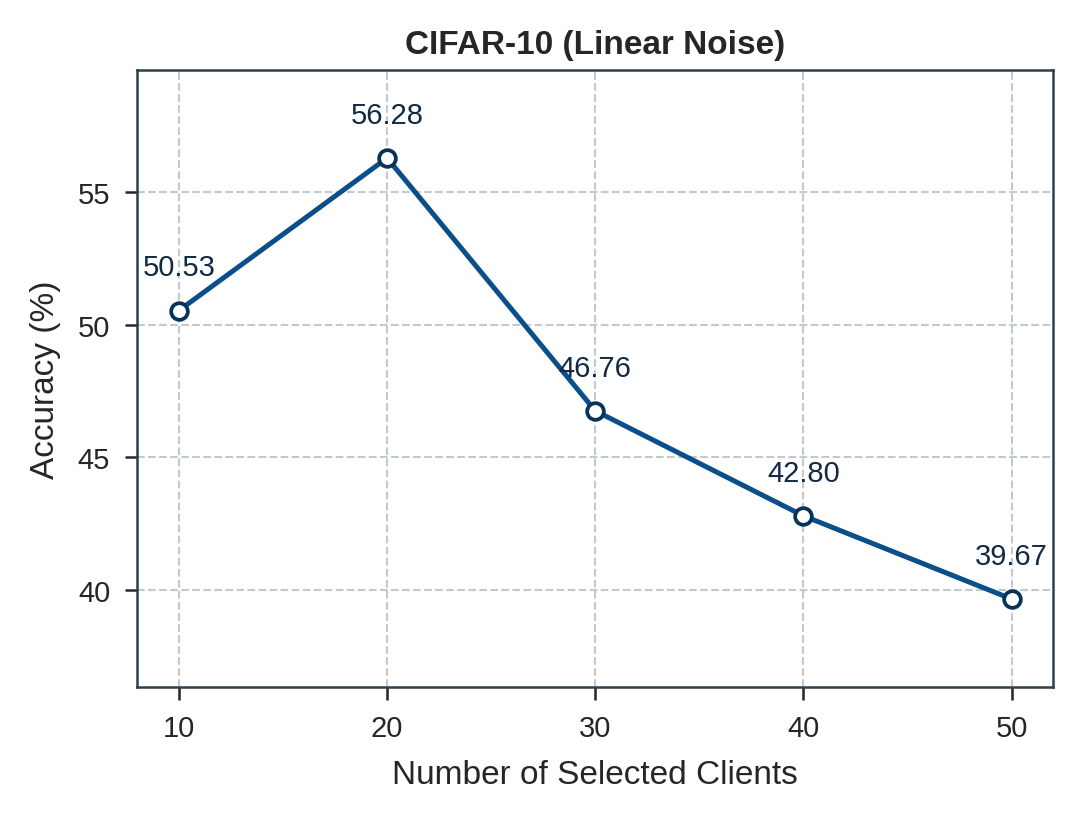
\includegraphics[width=0.31\textwidth]{figure/screening.png}
    \hfill
    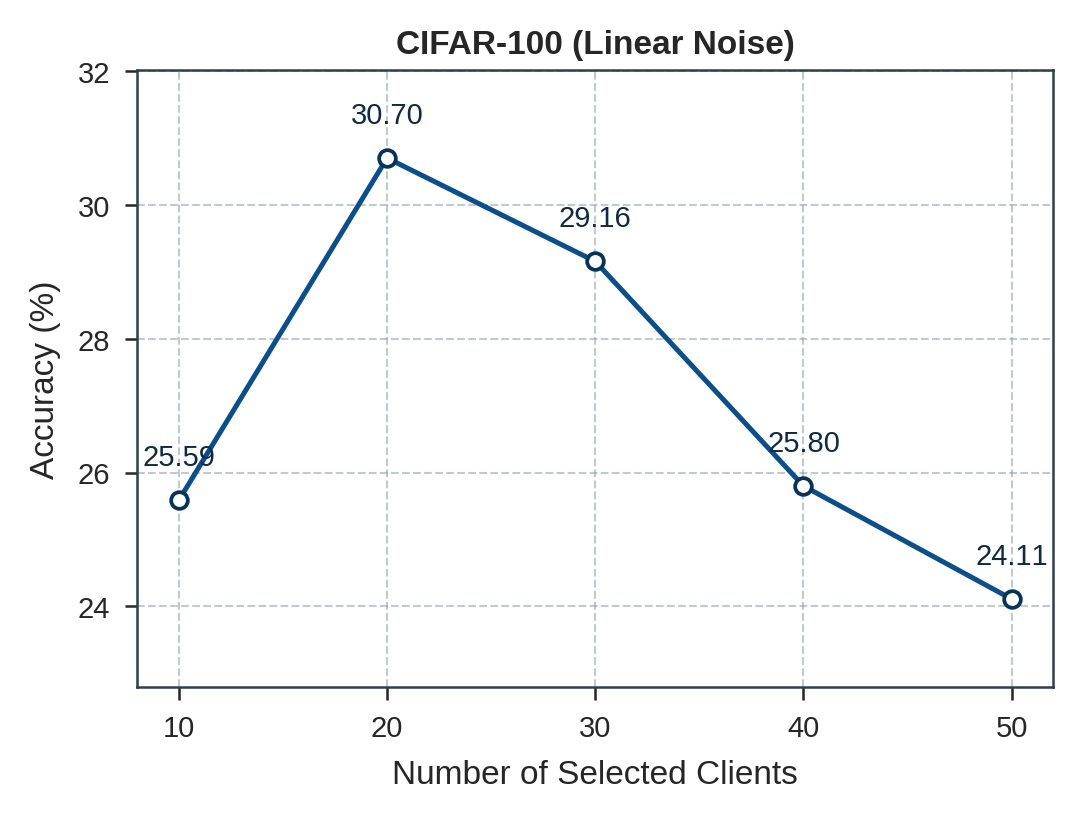
\includegraphics[width=0.31\textwidth]{figure/nips/scale/cifar100.png}
    \hfill
    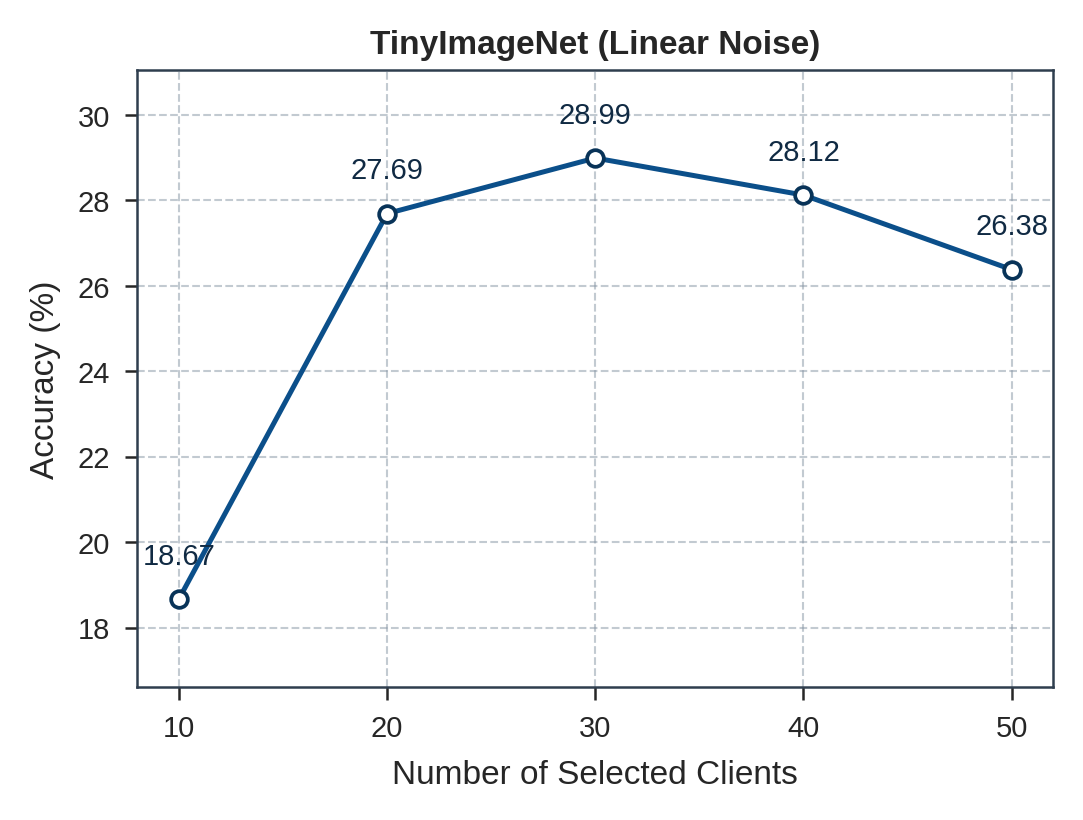
\includegraphics[width=0.31\textwidth]{figure/nips/scale/tinyimagenet.png}
    \caption{Effect of the selected client pool size on final test accuracy under coupled label noise and Non-IID heterogeneity on CIFAR-10, CIFAR-100, and TinyImageNet. Performance is non-monotonic with respect to the number of participating clients, showing that selecting an appropriate subset can outperform full participation.}
    \label{fig:screening}
\end{figure*}

\section{Additional Tables and Compatibility Results}
\label{app:additional_results}

\subsection{MedMNIST Non-IID Robustness}

Table~\ref{tab:medmnist_noniid_appendix} reports the MedMNIST counterpart of the Non-IID robustness experiment under linear heterogeneous noise.
The results show that the relative ranking is dataset dependent: FedRAA achieves the strongest accuracy at strong Non-IID, while FedNoRo and FedGreed are strongest at moderate and weak Non-IID levels, respectively.
This behavior is consistent with the role of the admission stage.
When heterogeneity is strong, filtering noisy and target-mismatched clients can provide a clearer benefit because full participation mixes highly incompatible local objectives.
When heterogeneity becomes weaker, the advantage shifts toward methods that exploit more participants during optimization.
Therefore, the MedMNIST appendix result should be read together with the cost analysis in the main text: FedRAA is designed to provide a reliable and efficient participant pool, rather than to maximize final accuracy in every single dataset column.

\begin{table}[t]
\centering
\caption{MedMNIST accuracy (\%) under linear noise with different Dirichlet Non-IID levels. Results use the same best-test-accuracy protocol as Table~\ref{tab:noisy_fl_accuracy} and are reported as mean$\pm$standard deviation. Best results are highlighted in bold and second-best results are underlined.}
\label{tab:medmnist_noniid_appendix}
\setlength{\tabcolsep}{5pt}
\renewcommand{\arraystretch}{1.10}
\begin{tabular}{lccc}
\toprule
\textbf{Method} & $\alpha=0.1$ & $\alpha=0.5$ & $\alpha=1.0$ \\
\midrule
All & 46.55$\pm$1.44 & 60.89$\pm$1.89 & 67.68$\pm$1.72 \\
RFA~\cite{pillutla2022robust} & 38.82$\pm$1.50 & 63.38$\pm$3.24 & 61.60$\pm$1.47 \\
FedGreed~\cite{kritharakis2025fedgreed} & 21.18$\pm$0.00 & \underline{83.09$\pm$3.17} & \textbf{89.33$\pm$2.27} \\
LASA~\cite{xu2025lasa} & 38.97$\pm$0.86 & 54.97$\pm$0.51 & 57.08$\pm$1.91 \\
FedNed~\cite{lu2024fedned} & 45.50$\pm$2.12 & 64.29$\pm$0.54 & 67.96$\pm$1.49 \\
FedNoRo~\cite{wu2023fednoro} & 33.92$\pm$2.13 & \textbf{85.48$\pm$0.41} & 78.07$\pm$0.51 \\
FedCorr~\cite{xu2022fedcorr} & 4.88$\pm$0.86 & 55.54$\pm$13.10 & 69.09$\pm$9.95 \\
FedCS~\cite{hao2025fedcs} & 24.66$\pm$1.40 & 56.60$\pm$3.02 & 79.06$\pm$1.39 \\
FedFixer~\cite{ji2024fedfixer} & \underline{46.72$\pm$1.47} & 61.06$\pm$1.92 & 67.85$\pm$1.75 \\
FedDiv~\cite{li2024feddiv} & 46.41$\pm$1.46 & 60.75$\pm$1.91 & 67.54$\pm$1.74 \\
\midrule
FedRAA (ours) & \textbf{47.71$\pm$1.08} & 81.05$\pm$0.80 & \underline{86.82$\pm$0.10} \\
\bottomrule
\end{tabular}
\end{table}

\subsection{Compatibility with Co-teach+}

Co-teach+ is applied during local training, while FedRAA acts before federated optimization by restricting the participant pool.
The two mechanisms are therefore complementary: FedRAA reduces the amount of noisy supervision entering the global process, and Co-teach+ further suppresses noisy examples within the admitted clients.
Table~\ref{tab:coteach_merged} shows that the combined variant improves the standalone methods in most settings, especially when the training-stage correction can operate on a cleaner and more representative admitted subset.

\begin{table*}[t]
\centering
\caption{Compatibility with Co-teach+ under heterogeneous noise. Results are mean accuracy (\%) over the converged stage. Best results are highlighted in bold, and second-best results are underlined.}
\label{tab:coteach_merged}
\setlength{\tabcolsep}{4pt}
\renewcommand{\arraystretch}{1.10}
\begin{tabular*}{\textwidth}{@{\extracolsep{\fill}}lccccccccc@{}}
\toprule
\multirow{2}{*}{Method}
& \multicolumn{3}{c}{CIFAR-10}
& \multicolumn{3}{c}{CIFAR-100}
& \multicolumn{3}{c}{Tiny-ImageNet} \\
\cmidrule(lr){2-4}\cmidrule(lr){5-7}\cmidrule(lr){8-10}
& Linear & 2-Ph. & 3-Ph.
& Linear & 2-Ph. & 3-Ph.
& Linear & 2-Ph. & 3-Ph. \\
\midrule
Co-teach+
& 50.2 & \underline{79.3} & 75.2
& 25.9 & \underline{46.6} & \underline{45.5}
& 24.6 & \underline{37.8} & 36.8 \\
FedRAA
& \underline{56.5} & 74.5 & \underline{75.9}
& \underline{30.6} & 39.1 & 40.2
& \textbf{27.8} & 36.3 & \textbf{38.0} \\
\midrule
FedRAA + Co-teach+
& \textbf{63.2} & \textbf{81.5} & \textbf{81.3}
& \textbf{34.2} & \textbf{47.4} & \textbf{47.4}
& \underline{27.2} & \textbf{38.4} & \textbf{38.0} \\
\bottomrule
\end{tabular*}
\vspace{2pt}
\parbox{0.95\textwidth}{\footnotesize
The improvement of FedRAA + Co-teach+ indicates that pre-training admission and training-stage sample filtering address different failure modes. FedRAA mainly removes unreliable clients from the participant pool, while Co-teach+ handles residual noisy labels among the admitted clients.}
\end{table*}


\subsection{Compatibility with Jo-CoR}

We further test compatibility with Jo-CoR, another training-stage noisy-label learning method.
The available Jo-CoR runs cover a smaller subset of settings, so this experiment is used as an auxiliary check rather than a full comparison.
The result suggests that not every local correction method automatically improves after admission: Jo-CoR slightly improves CIFAR-100 linear noise when combined with FedRAA, but does not improve CIFAR-10 linear noise.
This contrast emphasizes that FedRAA is a general admission layer, while the benefit of a specific training-stage correction depends on its interaction with the remaining local data distribution.
\begin{table*}[t]
\centering
\caption{Compatibility with Jo-CoR under heterogeneous real-imitation noise. Results are mean accuracy (\%) over the converged stage. Best results in each column are highlighted in bold, and the second-best results are underlined.}
\label{tab:jocor_merged}
\setlength{\tabcolsep}{4pt}
\renewcommand{\arraystretch}{1.10}
\begin{tabular*}{\textwidth}{@{\extracolsep{\fill}}lccccccccc@{}}
\toprule
\multirow{2}{*}{Method}
& \multicolumn{3}{c}{CIFAR-10}
& \multicolumn{3}{c}{CIFAR-100}
& \multicolumn{3}{c}{Tiny-ImageNet} \\
\cmidrule(lr){2-4}\cmidrule(lr){5-7}\cmidrule(lr){8-10}
& Linear & 2-Ph. & 3-Ph.
& Linear & 2-Ph. & 3-Ph.
& Linear & 2-Ph. & 3-Ph. \\
\midrule
Jo-CoR
& 41.5 & -- & --
& 30.7 & -- & --
& -- & -- & -- \\
FedRAA
& \underline{56.5} & 74.5 & \underline{75.9}
& \underline{30.6} & 39.1 & 40.2
& \textbf{27.8} & 36.3 & \textbf{38.0} \\
\midrule
FedRAA + Jo-CoR
& 54.3 & -- & --
& 30.8 & -- & --
& -- & -- & -- \\
\bottomrule
\end{tabular*}
\vspace{2pt}
\parbox{0.95\textwidth}{\footnotesize
Dashes denote settings not included in this auxiliary compatibility check. Compared with Co-teach+, Jo-CoR shows a more mixed interaction with FedRAA, which suggests that the admission stage should be viewed as complementary to, but not a replacement for, carefully chosen training-stage noise correction.}
\end{table*}

\end{document}
